% Options for packages loaded elsewhere
% Options for packages loaded elsewhere
\PassOptionsToPackage{unicode}{hyperref}
\PassOptionsToPackage{hyphens}{url}
\PassOptionsToPackage{dvipsnames,svgnames,x11names}{xcolor}
%
\documentclass[
  letterpaper,
  DIV=11,
  numbers=noendperiod]{scrartcl}
\usepackage{xcolor}
\usepackage{amsmath,amssymb}
\setcounter{secnumdepth}{-\maxdimen} % remove section numbering
\usepackage{iftex}
\ifPDFTeX
  \usepackage[T1]{fontenc}
  \usepackage[utf8]{inputenc}
  \usepackage{textcomp} % provide euro and other symbols
\else % if luatex or xetex
  \usepackage{unicode-math} % this also loads fontspec
  \defaultfontfeatures{Scale=MatchLowercase}
  \defaultfontfeatures[\rmfamily]{Ligatures=TeX,Scale=1}
\fi
\usepackage{lmodern}
\ifPDFTeX\else
  % xetex/luatex font selection
\fi
% Use upquote if available, for straight quotes in verbatim environments
\IfFileExists{upquote.sty}{\usepackage{upquote}}{}
\IfFileExists{microtype.sty}{% use microtype if available
  \usepackage[]{microtype}
  \UseMicrotypeSet[protrusion]{basicmath} % disable protrusion for tt fonts
}{}
\makeatletter
\@ifundefined{KOMAClassName}{% if non-KOMA class
  \IfFileExists{parskip.sty}{%
    \usepackage{parskip}
  }{% else
    \setlength{\parindent}{0pt}
    \setlength{\parskip}{6pt plus 2pt minus 1pt}}
}{% if KOMA class
  \KOMAoptions{parskip=half}}
\makeatother
% Make \paragraph and \subparagraph free-standing
\makeatletter
\ifx\paragraph\undefined\else
  \let\oldparagraph\paragraph
  \renewcommand{\paragraph}{
    \@ifstar
      \xxxParagraphStar
      \xxxParagraphNoStar
  }
  \newcommand{\xxxParagraphStar}[1]{\oldparagraph*{#1}\mbox{}}
  \newcommand{\xxxParagraphNoStar}[1]{\oldparagraph{#1}\mbox{}}
\fi
\ifx\subparagraph\undefined\else
  \let\oldsubparagraph\subparagraph
  \renewcommand{\subparagraph}{
    \@ifstar
      \xxxSubParagraphStar
      \xxxSubParagraphNoStar
  }
  \newcommand{\xxxSubParagraphStar}[1]{\oldsubparagraph*{#1}\mbox{}}
  \newcommand{\xxxSubParagraphNoStar}[1]{\oldsubparagraph{#1}\mbox{}}
\fi
\makeatother

\usepackage{color}
\usepackage{fancyvrb}
\newcommand{\VerbBar}{|}
\newcommand{\VERB}{\Verb[commandchars=\\\{\}]}
\DefineVerbatimEnvironment{Highlighting}{Verbatim}{commandchars=\\\{\}}
% Add ',fontsize=\small' for more characters per line
\usepackage{framed}
\definecolor{shadecolor}{RGB}{241,243,245}
\newenvironment{Shaded}{\begin{snugshade}}{\end{snugshade}}
\newcommand{\AlertTok}[1]{\textcolor[rgb]{0.68,0.00,0.00}{#1}}
\newcommand{\AnnotationTok}[1]{\textcolor[rgb]{0.37,0.37,0.37}{#1}}
\newcommand{\AttributeTok}[1]{\textcolor[rgb]{0.40,0.45,0.13}{#1}}
\newcommand{\BaseNTok}[1]{\textcolor[rgb]{0.68,0.00,0.00}{#1}}
\newcommand{\BuiltInTok}[1]{\textcolor[rgb]{0.00,0.23,0.31}{#1}}
\newcommand{\CharTok}[1]{\textcolor[rgb]{0.13,0.47,0.30}{#1}}
\newcommand{\CommentTok}[1]{\textcolor[rgb]{0.37,0.37,0.37}{#1}}
\newcommand{\CommentVarTok}[1]{\textcolor[rgb]{0.37,0.37,0.37}{\textit{#1}}}
\newcommand{\ConstantTok}[1]{\textcolor[rgb]{0.56,0.35,0.01}{#1}}
\newcommand{\ControlFlowTok}[1]{\textcolor[rgb]{0.00,0.23,0.31}{\textbf{#1}}}
\newcommand{\DataTypeTok}[1]{\textcolor[rgb]{0.68,0.00,0.00}{#1}}
\newcommand{\DecValTok}[1]{\textcolor[rgb]{0.68,0.00,0.00}{#1}}
\newcommand{\DocumentationTok}[1]{\textcolor[rgb]{0.37,0.37,0.37}{\textit{#1}}}
\newcommand{\ErrorTok}[1]{\textcolor[rgb]{0.68,0.00,0.00}{#1}}
\newcommand{\ExtensionTok}[1]{\textcolor[rgb]{0.00,0.23,0.31}{#1}}
\newcommand{\FloatTok}[1]{\textcolor[rgb]{0.68,0.00,0.00}{#1}}
\newcommand{\FunctionTok}[1]{\textcolor[rgb]{0.28,0.35,0.67}{#1}}
\newcommand{\ImportTok}[1]{\textcolor[rgb]{0.00,0.46,0.62}{#1}}
\newcommand{\InformationTok}[1]{\textcolor[rgb]{0.37,0.37,0.37}{#1}}
\newcommand{\KeywordTok}[1]{\textcolor[rgb]{0.00,0.23,0.31}{\textbf{#1}}}
\newcommand{\NormalTok}[1]{\textcolor[rgb]{0.00,0.23,0.31}{#1}}
\newcommand{\OperatorTok}[1]{\textcolor[rgb]{0.37,0.37,0.37}{#1}}
\newcommand{\OtherTok}[1]{\textcolor[rgb]{0.00,0.23,0.31}{#1}}
\newcommand{\PreprocessorTok}[1]{\textcolor[rgb]{0.68,0.00,0.00}{#1}}
\newcommand{\RegionMarkerTok}[1]{\textcolor[rgb]{0.00,0.23,0.31}{#1}}
\newcommand{\SpecialCharTok}[1]{\textcolor[rgb]{0.37,0.37,0.37}{#1}}
\newcommand{\SpecialStringTok}[1]{\textcolor[rgb]{0.13,0.47,0.30}{#1}}
\newcommand{\StringTok}[1]{\textcolor[rgb]{0.13,0.47,0.30}{#1}}
\newcommand{\VariableTok}[1]{\textcolor[rgb]{0.07,0.07,0.07}{#1}}
\newcommand{\VerbatimStringTok}[1]{\textcolor[rgb]{0.13,0.47,0.30}{#1}}
\newcommand{\WarningTok}[1]{\textcolor[rgb]{0.37,0.37,0.37}{\textit{#1}}}

\usepackage{longtable,booktabs,array}
\usepackage{calc} % for calculating minipage widths
% Correct order of tables after \paragraph or \subparagraph
\usepackage{etoolbox}
\makeatletter
\patchcmd\longtable{\par}{\if@noskipsec\mbox{}\fi\par}{}{}
\makeatother
% Allow footnotes in longtable head/foot
\IfFileExists{footnotehyper.sty}{\usepackage{footnotehyper}}{\usepackage{footnote}}
\makesavenoteenv{longtable}
\usepackage{graphicx}
\makeatletter
\newsavebox\pandoc@box
\newcommand*\pandocbounded[1]{% scales image to fit in text height/width
  \sbox\pandoc@box{#1}%
  \Gscale@div\@tempa{\textheight}{\dimexpr\ht\pandoc@box+\dp\pandoc@box\relax}%
  \Gscale@div\@tempb{\linewidth}{\wd\pandoc@box}%
  \ifdim\@tempb\p@<\@tempa\p@\let\@tempa\@tempb\fi% select the smaller of both
  \ifdim\@tempa\p@<\p@\scalebox{\@tempa}{\usebox\pandoc@box}%
  \else\usebox{\pandoc@box}%
  \fi%
}
% Set default figure placement to htbp
\def\fps@figure{htbp}
\makeatother


% definitions for citeproc citations
\NewDocumentCommand\citeproctext{}{}
\NewDocumentCommand\citeproc{mm}{%
  \begingroup\def\citeproctext{#2}\cite{#1}\endgroup}
\makeatletter
 % allow citations to break across lines
 \let\@cite@ofmt\@firstofone
 % avoid brackets around text for \cite:
 \def\@biblabel#1{}
 \def\@cite#1#2{{#1\if@tempswa , #2\fi}}
\makeatother
\newlength{\cslhangindent}
\setlength{\cslhangindent}{1.5em}
\newlength{\csllabelwidth}
\setlength{\csllabelwidth}{3em}
\newenvironment{CSLReferences}[2] % #1 hanging-indent, #2 entry-spacing
 {\begin{list}{}{%
  \setlength{\itemindent}{0pt}
  \setlength{\leftmargin}{0pt}
  \setlength{\parsep}{0pt}
  % turn on hanging indent if param 1 is 1
  \ifodd #1
   \setlength{\leftmargin}{\cslhangindent}
   \setlength{\itemindent}{-1\cslhangindent}
  \fi
  % set entry spacing
  \setlength{\itemsep}{#2\baselineskip}}}
 {\end{list}}
\usepackage{calc}
\newcommand{\CSLBlock}[1]{\hfill\break\parbox[t]{\linewidth}{\strut\ignorespaces#1\strut}}
\newcommand{\CSLLeftMargin}[1]{\parbox[t]{\csllabelwidth}{\strut#1\strut}}
\newcommand{\CSLRightInline}[1]{\parbox[t]{\linewidth - \csllabelwidth}{\strut#1\strut}}
\newcommand{\CSLIndent}[1]{\hspace{\cslhangindent}#1}



\setlength{\emergencystretch}{3em} % prevent overfull lines

\providecommand{\tightlist}{%
  \setlength{\itemsep}{0pt}\setlength{\parskip}{0pt}}



 


\KOMAoption{captions}{tableheading}
\makeatletter
\@ifpackageloaded{tcolorbox}{}{\usepackage[skins,breakable]{tcolorbox}}
\@ifpackageloaded{fontawesome5}{}{\usepackage{fontawesome5}}
\definecolor{quarto-callout-color}{HTML}{909090}
\definecolor{quarto-callout-note-color}{HTML}{0758E5}
\definecolor{quarto-callout-important-color}{HTML}{CC1914}
\definecolor{quarto-callout-warning-color}{HTML}{EB9113}
\definecolor{quarto-callout-tip-color}{HTML}{00A047}
\definecolor{quarto-callout-caution-color}{HTML}{FC5300}
\definecolor{quarto-callout-color-frame}{HTML}{acacac}
\definecolor{quarto-callout-note-color-frame}{HTML}{4582ec}
\definecolor{quarto-callout-important-color-frame}{HTML}{d9534f}
\definecolor{quarto-callout-warning-color-frame}{HTML}{f0ad4e}
\definecolor{quarto-callout-tip-color-frame}{HTML}{02b875}
\definecolor{quarto-callout-caution-color-frame}{HTML}{fd7e14}
\makeatother
\makeatletter
\@ifpackageloaded{caption}{}{\usepackage{caption}}
\AtBeginDocument{%
\ifdefined\contentsname
  \renewcommand*\contentsname{Table of contents}
\else
  \newcommand\contentsname{Table of contents}
\fi
\ifdefined\listfigurename
  \renewcommand*\listfigurename{List of Figures}
\else
  \newcommand\listfigurename{List of Figures}
\fi
\ifdefined\listtablename
  \renewcommand*\listtablename{List of Tables}
\else
  \newcommand\listtablename{List of Tables}
\fi
\ifdefined\figurename
  \renewcommand*\figurename{Figure}
\else
  \newcommand\figurename{Figure}
\fi
\ifdefined\tablename
  \renewcommand*\tablename{Table}
\else
  \newcommand\tablename{Table}
\fi
}
\@ifpackageloaded{float}{}{\usepackage{float}}
\floatstyle{ruled}
\@ifundefined{c@chapter}{\newfloat{codelisting}{h}{lop}}{\newfloat{codelisting}{h}{lop}[chapter]}
\floatname{codelisting}{Listing}
\newcommand*\listoflistings{\listof{codelisting}{List of Listings}}
\makeatother
\makeatletter
\makeatother
\makeatletter
\@ifpackageloaded{caption}{}{\usepackage{caption}}
\@ifpackageloaded{subcaption}{}{\usepackage{subcaption}}
\makeatother
\usepackage{bookmark}
\IfFileExists{xurl.sty}{\usepackage{xurl}}{} % add URL line breaks if available
\urlstyle{same}
\hypersetup{
  pdftitle={Multi-Period Models and Difference in Differences},
  colorlinks=true,
  linkcolor={blue},
  filecolor={Maroon},
  citecolor={Blue},
  urlcolor={Blue},
  pdfcreator={LaTeX via pandoc}}


\title{Multi-Period Models and Difference in Differences}
\usepackage{etoolbox}
\makeatletter
\providecommand{\subtitle}[1]{% add subtitle to \maketitle
  \apptocmd{\@title}{\par {\large #1 \par}}{}{}
}
\makeatother
\subtitle{Lecture 9 (R code)}
\author{}
\date{}
\begin{document}
\maketitle

% --- St Andrews brand colours for callout boxes ---
\definecolor{quarto-callout-note-color}{HTML}{007DC5}
\definecolor{quarto-callout-note-color-frame}{HTML}{007DC5}

\definecolor{quarto-callout-tip-color}{HTML}{00853F}
\definecolor{quarto-callout-tip-color-frame}{HTML}{00853F}

\definecolor{quarto-callout-caution-color}{HTML}{F5842B}
\definecolor{quarto-callout-caution-color-frame}{HTML}{F5842B}

\definecolor{quarto-callout-warning-color}{HTML}{EE312A}
\definecolor{quarto-callout-warning-color-frame}{HTML}{EE312A}

\definecolor{quarto-callout-important-color}{HTML}{7B439A}
\definecolor{quarto-callout-important-color-frame}{HTML}{7B439A}

% This approach is similar to: https://github.com/orgs/quarto-dev/discussions/13739; which added the following to the YAML section 
%  pdf:
%    include-before-body:
%      - text: |
%          \definecolor{quarto-callout-note-color}{HTML}{007DC5}
%          \definecolor{quarto-callout-tip-color}{HTML}{00853F}
%          \definecolor{quarto-callout-important-color}{HTML}{7B439A}
%          \definecolor{quarto-callout-caution-color}{HTML}{F5842B}
%          \definecolor{quarto-callout-warning-color}{HTML}{EE312A}
 
% But follows the advice of https://quarto.org/docs/output-formats/pdf-basics.html to add macros.tex section. 

% Alternatively, you follow this approach: https://enrico.spinielli.net/posts/2023-05-01-quarto-callout-hack/
% However, it edits the formatting of the PDF entirely instead of just adding a few changes. 
% If following this advice, you append the above to the end of the title.tex file. 


\renewcommand*\contentsname{Table of contents}
{
\hypersetup{linkcolor=}
\setcounter{tocdepth}{3}
\tableofcontents
}

\section{Data Structure \& Notation}\label{data-structure-notation}

\subsection{Notation}\label{notation}

When we write down a linear regression model for a either a repeated
cross section or panel dataset, we add both \(i\) and \(t\) to the
subscripts:

\[
  y_{it} = \beta_0 + \beta_1 x_{it1} + \beta_2 x_{it2} + \dots + \beta_k x_{itk} + u_{it}
\]

However, you may also have some variables that

\begin{itemize}
\item
  do not vary with time: \(x_{i}\)

  \begin{itemize}
  \tightlist
  \item
    e.g.~individual ethnicity
  \end{itemize}
\item
  vary only with time: \(x_{t}\)

  \begin{itemize}
  \tightlist
  \item
    e.g.~adding aggregate unemployment rate to individual level model of
    wages
  \end{itemize}
\end{itemize}

\section{Pooled Cross Sections}\label{pooled-cross-sections}

\subsection{Hypothetical example: Poverty \&
SCP}\label{hypothetical-example-poverty-scp}

Suppose, a researcher wants to evaluate the impact that of the
\href{https://www.homeenergyscotland.org/home-energy-scotland-grant-loan}{Home
Energy Scotland Grant and Loan} programme on a household's energy
expenditure.

\begin{itemize}
\tightlist
\item
  Grant of up to £7,500 to install clean heating systems and energy
  efficiency measures.
\end{itemize}

\begin{center}
\pandocbounded{
\includegraphics[keepaspectratio]{material/lecture-9/home-energy-scotland.png}}
\end{center}

\subsection{Empirical specification}\label{empirical-specification}

They propose the following linear regression model specification

\[
  energy_{it} = \delta + \beta grant_{it} + \mathbf{x}_{it}\gamma + \varepsilon_{it}
\]

To be estimated using repeated cross sections of the Scottish Household
Survey.

\begin{itemize}
\item
  \(energy_{it}\): amount (£'s) spent on energy
\item
  \(grant_{it}\): cumulative amount received from the programme
\end{itemize}

\subsection{Controls}\label{controls}

As controls, the author collects information at the household level
(\(\mathbf{x}_{it}\)) on:

\begin{enumerate}
\def\labelenumi{\arabic{enumi}.}
\item
  dwelling type
\item
  ownership type
\item
  household size
\item
  household income
\item
  number of rooms
\item
  location
\end{enumerate}

\subsection{Time-varying factors}\label{time-varying-factors}

But there are other key macroeconomics variables that explain
expenditure on energy over time:

\begin{enumerate}
\def\labelenumi{\arabic{enumi}.}
\item
  Global oil price
\item
  Global gas price
\item
  Domestic energy prices (gas,electricity)

  \begin{itemize}
  \tightlist
  \item
    Determined by domestic auctions: marginal supplier
  \end{itemize}
\end{enumerate}

This variables vary with time, but NOT across households:

\[
  \mathbf{z}_t\eta
\]

\subsection{}\label{section}

So, our model is actually,

\[
  energy_{it} = \delta + \beta grant_{it} + \mathbf{x}_{it}\gamma + \mathbf{z}_t\eta + \varepsilon_{it}
\]

where,

\begin{itemize}
\item
  \(\mathbf{x}\) includes household level controls
\item
  \(\mathbf{z}\) includes time-varying (macroeconomic/aggregate)
  controls
\end{itemize}

\subsection{Identification}\label{identification}

Since the data comprises repeated cross sections of individual, it is
reasonable to assume that each observation is a random draw from the
underlying population (MLR 2).

\hfill\break

\begin{itemize}
\item
  As before, we need MLR1-4a for consistency.
\item
  The question is more whether MLR 1 holds true across time.

  \begin{itemize}
  \tightlist
  \item
    Is the model time-invariant?
  \end{itemize}
\end{itemize}

\subsection{Time-varying parameters}\label{time-varying-parameters}

We could evaluate this question using a Chow test:

\begin{itemize}
\tightlist
\item
  Estimate the model separately for each year:
\end{itemize}

\[
  energy_{it} = \delta_t + \beta_t grant_{it} + \mathbf{x}_{it}\gamma_t + \mathbf{z}_t\eta_t + \varepsilon_{it} \quad \text{for}\;t = 1,\dots,T
\]

\begin{itemize}
\tightlist
\item
  Test whether the parameters vary using \(SSR_t\) from each equation.
\end{itemize}

\subsection{}\label{section-1}

\textbf{BUT} there is a problem with \(\mathbf{z}_t\eta_t\) in this
model:

\begin{itemize}
\item
  In any given period, these variables do not vary

  \begin{itemize}
  \item
    e.g., oil price is \$100 in period \(t=1\) and \$120 for period
    \(t=2\)
  \item
    but within a given period \(t\), the oil price doesn't vary across
    households
  \end{itemize}
\item
  So, \(\mathbf{z}_t\eta_t\) is a constant in each individual cross
  section

  \begin{itemize}
  \tightlist
  \item
    cannot be separately identified from \(\delta_t\), the time-varying
    constant
  \end{itemize}
\end{itemize}

\subsection{Time fixed effects}\label{time-fixed-effects}

If we take our original model and allow the constant term (only) to vary
with time.

\[
  energy_{it} = \delta_t + \beta grant_{it} + \mathbf{x}_{it}\gamma + \varepsilon_{it}
\]

then we must exclude all variables that also vary \emph{only} with time:
\(\mathbf{z}_t\eta\)

\begin{itemize}
\item
  We call \(\delta_t\) \textbf{time fixed effects}
\item
  These time FEs ``absorb'' any other variables that vary only with
  time.
\item
  We say, time FEs ``control'' for any time-varying (e.g.,
  macroeconomic) factors/shocks; \textbf{even ones we don't observe} in
  the data.
\end{itemize}

\subsection{Time dummies:}\label{time-dummies}

When it comes to estimation, time FEs are equvilent to including a set
of dummy variables: one for each year.

\[
  \delta_t = \sum_{j=1}^{T}\delta_j \mathbf{1}\{j=t\} 
\]

In place of a constant, we have \(T\) dummy variables that identify each
period.

\begin{itemize}
\tightlist
\item
  For any given \(t\), only one of these dummies \(=1\)
\end{itemize}

\begin{tcolorbox}[enhanced jigsaw, opacitybacktitle=0.6, colbacktitle=quarto-callout-note-color!10!white, rightrule=.15mm, colframe=quarto-callout-note-color-frame, bottomtitle=1mm, breakable, leftrule=.75mm, colback=white, toprule=.15mm, toptitle=1mm, left=2mm, title=\textcolor{quarto-callout-note-color}{\faInfo}\hspace{0.5em}{Note}, coltitle=black, arc=.35mm, titlerule=0mm, bottomrule=.15mm, opacityback=0]

This notation can be very confusing. Do not concern yourself with the
complicated sum, but rather the intuition that when we include an
intercept in a linear regression it gives us the slope coefficient on a
constant (a regressor that \(=1\) for all observations). To implement
time FEs, we are essentially adding a separate constant for each period
time. And these constants are all just dummy variables:
\(\mathbf{1}\{j=t\}\).

\end{tcolorbox}

\section{Panel Models}\label{panel-models}

\subsection{Preamble}\label{preamble}

There is a large, fairly complex literature on panel data models:

\begin{itemize}
\item
  Static vs Dynamic models
\item
  Short (small \(T\)) vs long (large \(T\)) panels
\item
  Variance (standard error) corrections for autocorrelation
\end{itemize}

We are going to skip over many of these topics, to talk about the types
of panel data models you might see in modern applied (microeconomic)
research

\begin{itemize}
\tightlist
\item
  short, static panel data models
\end{itemize}

\subsection{Identification}\label{identification-1}

As with cross sectional models, the primary concern is the potential
endogeneity of the regressors:

\[
  Cov(\varepsilon_{it},x_{itj}) \quad j=1,\dots,k 
\]

\subsection{Composite error}\label{composite-error}

What's different in panel data is the opportunity to consider a
composite error:

\[
  \varepsilon_{it}= \nu_{i}+\upsilon_{it}
\]

where,

\begin{itemize}
\item
  \(\nu_{i}\): time-invariant heterogeneity

  \begin{itemize}
  \tightlist
  \item
    e.g., unobserved household preferences for heating of the home.
  \end{itemize}
\item
  \(\upsilon_{it}\): time-varying unobserved heterogeneity (``shocks'')

  \begin{itemize}
  \tightlist
  \item
    e.g., a household is away and turns off their heating for a month
  \end{itemize}
\end{itemize}

\subsection{}\label{section-2}

It is likely that time-invariant heterogeneity (\(\nu_{i}\)) is related
to many observed regressors. For example,

\[
  Cov(\nu_{i}, grant_{it}) \neq 0
\]

\begin{itemize}
\item
  households with a strong environmental preferences are more likely to
  apply for a grant to investment in solar panels.

  \begin{itemize}
  \tightlist
  \item
    This would be a problem of ``selection on unobservables''
  \end{itemize}
\end{itemize}

\textbf{Fortunatley}, we are going to investigate an estimation
procedure that eliminates \(\nu_i\) from the equation. So, we only need
to concern ourselves with MLR 4a w.r.t. \(\upsilon_{it}\).

\[
  Cov(\upsilon_{it}, x_{itj}) = 0 \quad j=1,\dots,k
\]

\subsection{Autocorrelation}\label{autocorrelation}

A secondary concern relates to the correlation of \(\varepsilon_{it}\)
across observations in panel data.

\begin{itemize}
\item
  Suppose we remove \(\nu_{i}\) from the model
\item
  We must expect that

  \[
    Cov(\upsilon_{it},\upsilon_{is}) \neq 0 \quad \text{for}\; t\neq s
  \]

  \begin{itemize}
  \tightlist
  \item
    Issue for estimation of variance.
  \item
    We fix this by estimating clustered SEs (at the unit level)
  \end{itemize}
\end{itemize}

\subsection{Example}\label{example}

Consider our model:

\[
  energy_{it} = \delta_t + \beta grant_{it} + \mathbf{x}_{it}\gamma + \varepsilon_{it}
\]

Some of the household characteristics in \(\mathbf{x}_{it}\) may not
vary with time:

\begin{enumerate}
\def\labelenumi{\arabic{enumi}.}
\item
  dwelling type (might not)
\item
  ownership type (might not)
\item
  household size (might not)
\item
  household income (probably does)
\item
  number of rooms (might not)
\item
  location (might not)
\end{enumerate}

\textbf{What really matters is whether they vary in the data.}

\subsection{Time-invarianct
covariates}\label{time-invarianct-covariates}

Let's split up the household characteristics into

\begin{itemize}
\item
  those that vary with time: \(\mathbf{x}_{it}\gamma_1\)
\item
  those that are time-invariant: \(\mathbf{x}_{i}\gamma_2\)
\end{itemize}

\[
  energy_{it} = \delta_t + \beta grant_{it} + \mathbf{x}_{it}\gamma_1 + \mathbf{x}_{i}\gamma_2 + \varepsilon_{it}
\]

\subsection{Unit FEs}\label{unit-fes}

Because we observe repeated observations of the \textbf{same} household,
we can include unit FEs

\[
  energy_{it} = \alpha_i + \delta_t + \beta grant_{it} + \mathbf{x}_{it}\gamma_1 + \varepsilon_{it}
\]

\textbf{BUT} by the same logic as before,

\begin{itemize}
\item
  unit FEs ``absorb'' anything that is invariant at the unit level:
  \(\mathbf{x}_{i}\gamma_2\)
\item
  we say, unit FEs ``control'' for any time-invariant (e.g., fixed
  building characteristics) heterogeneity (i.e.~things that vary across
  \(i\)); \textbf{even ones we don't observe} in the data.

  \begin{itemize}
  \tightlist
  \item
    unit FEs potentially control for things we do not observe:
    e.g.~household preferences over how warm to keep their home.
  \end{itemize}
\end{itemize}

\subsection{Time-varying treatment}\label{time-varying-treatment}

Crucially, this means that the treatment variable \(grant_{it}\) must
vary at the \textbf{unit-level over time}.

\[
  energy_{it} = \alpha_i + \delta_t + \beta grant_{it} + \mathbf{x}_{it}\gamma_1 + \varepsilon_{it}
\]

for example, a households (cumulative) grant is looks like over 4
periods

\[
  grant_{i} = \{0,0,3000,7500\}
\]

\subsection{Estimation}\label{estimation}

The OLS estimator for this model is often referred to as the
``fixed-effects'' (or ``within'') estimator. The logic is that you
estimate a transformed version of the model:

\[
  \widetilde{energy}_{it} = \delta_t + \beta \widetilde{grant}_{it} + \widetilde{\mathbf{x}}_{it}\gamma_1 + \tilde{\upsilon}_{it}
\]

where each variable has been demeaned at the \textbf{unit-level}

\[
  \widetilde{energy}_{it} = energy_{it} - \overline{energy}_{i}
\]

\begin{itemize}
\item
  Remember: when you include a constant in the model it does the same
  thing, but using the global mean of the variable.
\item
  Helps with the intuition of why the remaining variables must vary at
  the unit level over time.
\item
  The error term is \(\tilde{\upsilon}_{it}\) because
  \(\varepsilon_{it} = \nu_{i}+\upsilon_{it}\) and \(\nu_{i}\) is
  time-invariant:
\end{itemize}

\[
    \tilde{\varepsilon}_{it} = \tilde{\upsilon}_{it}
  \]

\section{Data Example: EVs \& PM2.5}\label{data-example-evs-pm2.5}

\subsection{Data}\label{data}

Unfortunately, we do not have data on these hypothetical grants.

\begin{itemize}
\tightlist
\item
  Data on EV vehicle registration and neighbourhood PM2.5 from
  \href{lecture-4-multi.qmd}{Lecture 4}
\end{itemize}

\[
  \ln(PM2.5_{\ell,t}) = \delta_t + \beta EVshare_{\ell,t} + \gamma \ln(pop_{\ell,t}) + u_{\ell,t}
\]

\begin{verbatim}
       year |      Freq.     Percent        Cum.
------------+-----------------------------------
       2018 |        285       14.29       14.29
       2019 |        285       14.29       28.57
       2020 |        285       14.29       42.86
       2021 |        285       14.29       57.14
       2022 |        285       14.29       71.43
       2023 |        285       14.29       85.71
       2024 |        285       14.29      100.00
------------+-----------------------------------
      Total |      1,995      100.00
\end{verbatim}

\subsection{Pooled cross section}\label{pooled-cross-section}

\begin{Shaded}
\begin{Highlighting}[]
\CommentTok{\# Load the Stata file}
\NormalTok{pm25\_panel }\OtherTok{\textless{}{-}} \FunctionTok{read.csv}\NormalTok{(}\FunctionTok{file.path}\NormalTok{(data\_dir, }\StringTok{"pm25\_panel.csv"}\NormalTok{))}

\CommentTok{\# Estimate univariate linear regression}
\NormalTok{model1 }\OtherTok{\textless{}{-}} \FunctionTok{lm}\NormalTok{(ln\_pm25 }\SpecialCharTok{\textasciitilde{}}\NormalTok{ ev\_share, }\AttributeTok{data =}\NormalTok{ pm25\_panel)}
\NormalTok{model2 }\OtherTok{\textless{}{-}} \FunctionTok{lm}\NormalTok{(ln\_pm25 }\SpecialCharTok{\textasciitilde{}}\NormalTok{ ev\_share }\SpecialCharTok{+}\NormalTok{ ln\_pop, }\AttributeTok{data =}\NormalTok{ pm25\_panel)}
\NormalTok{model3 }\OtherTok{\textless{}{-}} \FunctionTok{lm}\NormalTok{(ln\_pm25 }\SpecialCharTok{\textasciitilde{}}\NormalTok{ ev\_share }\SpecialCharTok{+}\NormalTok{ ln\_pop }\SpecialCharTok{+} \FunctionTok{factor}\NormalTok{(year), }\AttributeTok{data =}\NormalTok{ pm25\_panel)}

\CommentTok{\# View results}
\FunctionTok{modelsummary}\NormalTok{(}\FunctionTok{list}\NormalTok{(}\StringTok{"(1)"} \OtherTok{=}\NormalTok{ model1, }\StringTok{"(2)"} \OtherTok{=}\NormalTok{ model2, }\StringTok{"(3)"} \OtherTok{=}\NormalTok{ model3))}
\end{Highlighting}
\end{Shaded}

\begin{table}
\centering
\begin{tblr}[         %% tabularray outer open
]                     %% tabularray outer close
{                     %% tabularray inner open
colspec={Q[]Q[]Q[]Q[]},
hline{2}={1-4}{solid, black, 0.05em},
hline{20}={1-4}{solid, black, 0.05em},
hline{1}={1-4}{solid, black, 0.08em},
hline{28}={1-4}{solid, black, 0.08em},
column{2-4}={}{halign=c},
column{1}={}{halign=l},
}                     %% tabularray inner close
& (1) & (2) & (3) \\
(Intercept) & \num{2.053} & \num{1.330} & \num{1.477} \\
& (\num{0.005}) & (\num{0.088}) & (\num{0.067}) \\
ev\_share & \num{-0.441} & \num{-0.494} & \num{1.736} \\
& (\num{0.200}) & (\num{0.197}) & (\num{0.166}) \\
ln\_pop &  & \num{0.061} & \num{0.063} \\
&  & (\num{0.007}) & (\num{0.006}) \\
factor(year)2019 &  &  & \num{0.006} \\
&  &  & (\num{0.013}) \\
factor(year)2020 &  &  & \num{-0.244} \\
&  &  & (\num{0.013}) \\
factor(year)2021 &  &  & \num{-0.274} \\
&  &  & (\num{0.013}) \\
factor(year)2022 &  &  & \num{-0.241} \\
&  &  & (\num{0.013}) \\
factor(year)2023 &  &  & \num{-0.347} \\
&  &  & (\num{0.013}) \\
factor(year)2024 &  &  & \num{-0.353} \\
&  &  & (\num{0.013}) \\
Num.Obs. & \num{1995} & \num{1995} & \num{1995} \\
R2 & \num{0.002} & \num{0.035} & \num{0.448} \\
R2 Adj. & \num{0.002} & \num{0.034} & \num{0.446} \\
AIC & \num{-711.6} & \num{-776.3} & \num{-1878.7} \\
BIC & \num{-694.8} & \num{-753.9} & \num{-1822.7} \\
Log.Lik. & \num{358.792} & \num{392.138} & \num{949.335} \\
F & \num{4.859} & \num{36.369} & \num{201.591} \\
RMSE & \num{0.20} & \num{0.20} & \num{0.15} \\
\end{tblr}
\end{table}

\subsection{Panel}\label{panel}

\begin{Shaded}
\begin{Highlighting}[]
\KeywordTok{est} \KeywordTok{clear}
\KeywordTok{qui} \KeywordTok{reg}\NormalTok{ ln\_pm25 ev\_share }
    \KeywordTok{est} \KeywordTok{store}\NormalTok{ model1}
\KeywordTok{qui} \KeywordTok{reg}\NormalTok{ ln\_pm25 ev\_share ln\_pop}
    \KeywordTok{est} \KeywordTok{store}\NormalTok{ model2}
\KeywordTok{qui} \KeywordTok{reg}\NormalTok{ ln\_pm25 ev\_share ln\_pop i.}\FunctionTok{year}
    \KeywordTok{est} \KeywordTok{store}\NormalTok{ model3}
\KeywordTok{qui} \KeywordTok{areg}\NormalTok{ ln\_pm25 ev\_share ln\_pop i.}\FunctionTok{year}\NormalTok{, absorb(la\_id)}
    \KeywordTok{est} \KeywordTok{store}\NormalTok{ model4}
\NormalTok{etable, }\KeywordTok{est}\NormalTok{(model1 model2 model3 model4)}
\end{Highlighting}
\end{Shaded}

\begin{verbatim}
                       ln_pm25 ln_pm25 ln_pm25 ln_pm25
------------------------------------------------------
ev_share                -0.441  -0.494   1.736  -0.160
                       (0.200) (0.197) (0.166) (0.130)
ln_pop                           0.061   0.063   0.141
                               (0.007) (0.006) (0.094)
year                                                  
  2019                                   0.006   0.008
                                       (0.013) (0.006)
  2020                                  -0.244  -0.237
                                       (0.013) (0.006)
  2021                                  -0.274  -0.259
                                       (0.013) (0.007)
  2022                                  -0.241  -0.216
                                       (0.013) (0.007)
  2023                                  -0.347  -0.311
                                       (0.013) (0.008)
  2024                                  -0.353  -0.303
                                       (0.013) (0.008)
Intercept                2.053   1.330   1.477   0.554
                       (0.005) (0.088) (0.067) (1.122)
Number of observations    1995    1995    1995    1995
------------------------------------------------------
\end{verbatim}

\subsection{Unit FEs}\label{unit-fes-1}

Modern FEs function \texttt{reghdfe}

\begin{Shaded}
\begin{Highlighting}[]
\CommentTok{\# Load the fixest package}
\FunctionTok{library}\NormalTok{(}\StringTok{"fixest"}\NormalTok{)}

\CommentTok{\# Estimate model with two{-}way FEs}
\NormalTok{model4 }\OtherTok{\textless{}{-}} \FunctionTok{feols}\NormalTok{(ln\_pm25 }\SpecialCharTok{\textasciitilde{}}\NormalTok{ ev\_share }\SpecialCharTok{+}\NormalTok{ ln\_pop }\SpecialCharTok{|}\NormalTok{ la\_id }\SpecialCharTok{+}\NormalTok{ year, }\AttributeTok{data =}\NormalTok{ pm25\_panel)}

\CommentTok{\# View results}
\FunctionTok{summary}\NormalTok{(model4)}
\end{Highlighting}
\end{Shaded}

\begin{verbatim}
OLS estimation, Dep. Var.: ln_pm25
Observations: 1,995
Fixed-effects: la_id: 285,  year: 7
Standard-errors: IID 
          Estimate Std. Error  t value Pr(>|t|) 
ev_share -0.160365   0.129938 -1.23417  0.21731 
ln_pop    0.140789   0.093979  1.49809  0.13430 
---
Signif. codes:  0 '***' 0.001 '**' 0.01 '*' 0.05 '.' 0.1 ' ' 1
RMSE: 0.070215     Adj. R2: 0.858989
                 Within R2: 0.001908
\end{verbatim}

\section{Difference in Differences}\label{difference-in-differences}

\subsection{2 groups}\label{groups}

In experiments (\href{lecture-6-multi.qmd}{lecture 6}), we compare two
groups

\[
  E[y_i | w_i =1]-E[y_i|w_i=0]
\]

And \emph{under unconfoundedness} (whether by randomization or
assumption),

\[
  =E[y_i(1)-y_i(0)] = \tau_{ate}
\]

\subsection{2 groups, 2 periods}\label{groups-2-periods}

Suppose we observe 2 groups, across 2 periods of time:

\[
  y_{it}
\]

\begin{itemize}
\item
  we must have either a repeated cross section or a panel
\item
  be able to follow the same group in each period
\end{itemize}

\subsection{Treatment}\label{treatment}

Let us consider a discrete treatment, denoted:\footnote{Distinguishing
  from \(w_i\), which is associated with an (conditionally) unconfounded
  assignment. Here \(d_i\) need not be unconfounded.}

\[
  d_i = \mathbf{1}\{\text{treated}\}
\]

\hfill\break

\emph{Crucially}, we observe the treated (\(d_i=1\)) and control
(\(d_i=0\)) groups \textbf{before and after} the treatment.

Let,

\[
  q_t = \mathbf{1}\{t>t_0\}
\]

where \(t_0\) is the period of treatment.

\subsection{Post period}\label{post-period}

In the period immediately after the treatment, you can identify

\[
  E[y_{it} | d_i =1, q_t = 1]-E[y_{it} | d_i =0, q_t = 1]
\]

Written in terms of POs, this gives you

\[
  E[y_{it}(1) | d_i =1, q_t = 1]-E[y_{it}(0) | d_i =0, q_t = 1]
\]

\subsection{Decomposition}\label{decomposition}

We know from \href{lecture-6-multi.qmd}{Lecture 6}, that this difference
can be decomposed:

\[
  \begin{aligned}
  &E[y_{it}(1) | d_i =1, q_t = 1]-E[y_{it}(0) | d_i =0, q_t = 1] \\
  =& E[y_{it}(1) | d_i =1, q_t = 1]-\textcolor{red}{E[y_{it}(0) | d_i =1, q_t = 1]} \\
  &+\textcolor{red}{E[y_{it}(0) | d_i =1, q_t = 1]} -E[y_{it}(0) | d_i =0, q_t = 1] \\
  =& \underbrace{E[y_{it}(1)-y_{it}(0) | d_i =1, q_t = 1]}_{\tau_{att}} \\
  &+\underbrace{\textcolor{red}{E[y_{it}(0) | d_i =1, q_t = 1]} -E[y_{it}(0) | d_i =0, q_t = 1]}_\text{Selection}
  \end{aligned}
\]

\subsection{Pre period}\label{pre-period}

In the period immediately before the treatment, you can identify

\[
  \textcolor{blue}{E[y_{it} | d_i =1, q_t = 0]-E[y_{it} | d_i =0, q_t = 0]}
\]

Since neither group is yet treated, this gives you

\[
  \textcolor{blue}{E[y_{it}(0) | d_i =1, q_t = 0]-E[y_{it}(0) | d_i =0, q_t = 0]}
\]

\begin{itemize}
\item
  \textbf{Assumes:} treated group do not anticipate the treatment
\item
  We call this \textbf{no anticipation} (or no pre-emptive behaviour)
  assumption
\end{itemize}

\subsection{}\label{section-3}

Compare this term from the pre-period:

\[
  \textcolor{blue}{E[y_{it}(0) | d_i =1, q_t = 0]-E[y_{it}(0) | d_i =0, q_t = 0]}
\]

\hfill\break

With the selection term from the post period:

\[
  \textcolor{red}{E[y_{it}(0) | d_i =1, q_t = 1]} -E[y_{it}(0) | d_i =0, q_t = 1]
\]

\subsection{}\label{section-4}

What if we deduct one difference from the other:

\[
  \begin{aligned}
  &\big[E[y_{it} | d_i =1, q_t = 1]-E[y_{it} | d_i =0, q_t = 1]\big] \\
  &-\big[\textcolor{blue}{E[y_{it} | d_i =1, q_t = 0]-E[y_{it} | d_i =0, q_t = 0]}\big] 
  \end{aligned}
\]

a \textbf{difference in differences}

\subsection{Decomposition}\label{decomposition-1}

Following the same decomposition, you end up with:

\[
  \begin{aligned}
   & \underbrace{E[y_{it}(1)-y_{it}(0) | d_i =1, q_t = 1]}_{\tau_{att}} \\
  &+\big[\textcolor{red}{E[y_{it}(0) | d_i =1, q_t = 1]} -E[y_{it}(0) | d_i =0, q_t = 1]\big] \\
  &-\big[\textcolor{blue}{E[y_{it}(0) | d_i =1, q_t = 0]-E[y_{it}(0) | d_i =0, q_t = 0]}\big] \\
  =& \tau_{att}
  \end{aligned}
\]

\textbf{if we assume} the two terms middle differences (w.r.t. \(y(0)\))
are the same.

\subsection{Assumption}\label{assumption}

What is this assumption:

\[
  \begin{aligned}
   &\textcolor{red}{E[y_{it}(0) | d_i =1, q_t = 1]} -E[y_{it}(0) | d_i =0, q_t = 1] \\
  =&\textcolor{blue}{E[y_{it}(0) | d_i =1, q_t = 0]-E[y_{it}(0) | d_i =0, q_t = 0]}
  \end{aligned}
\]

\begin{itemize}
\tightlist
\item
  Selection term in pre-period is same as that in post-period.
\end{itemize}

\subsection{Parallel trends}\label{parallel-trends}

This can be re-arranged:

\[
  \begin{aligned}
   &\textcolor{red}{E[y_{it}(0) | d_i =1, q_t = 1]} - \textcolor{blue}{E[y_{it}(0) | d_i =1, q_t = 0]}  \\
  =&E[y_{it}(0) | d_i =0, q_t = 1]-\textcolor{blue}{E[y_{it}(0) | d_i =0, q_t = 0]}
  \end{aligned}
\]

\textbf{parallel trends assumption}

\begin{itemize}
\item
  in the absence of treatment, the mean of the 2 groups would change by
  the same amount.
\item
  this is very different to the assumption of unconfoundedness, which
  says:
  \(\textcolor{red}{E[y_{it}(0) | d_i =1, q_t = 1]} = \textcolor{blue}{E[y_{it}(0) | d_i =1, q_t = 0]}\)
\end{itemize}

\section{Graphical demonstration}\label{graphical-demonstration}

\subsection{Control group}\label{control-group}

\begin{center}
\pandocbounded{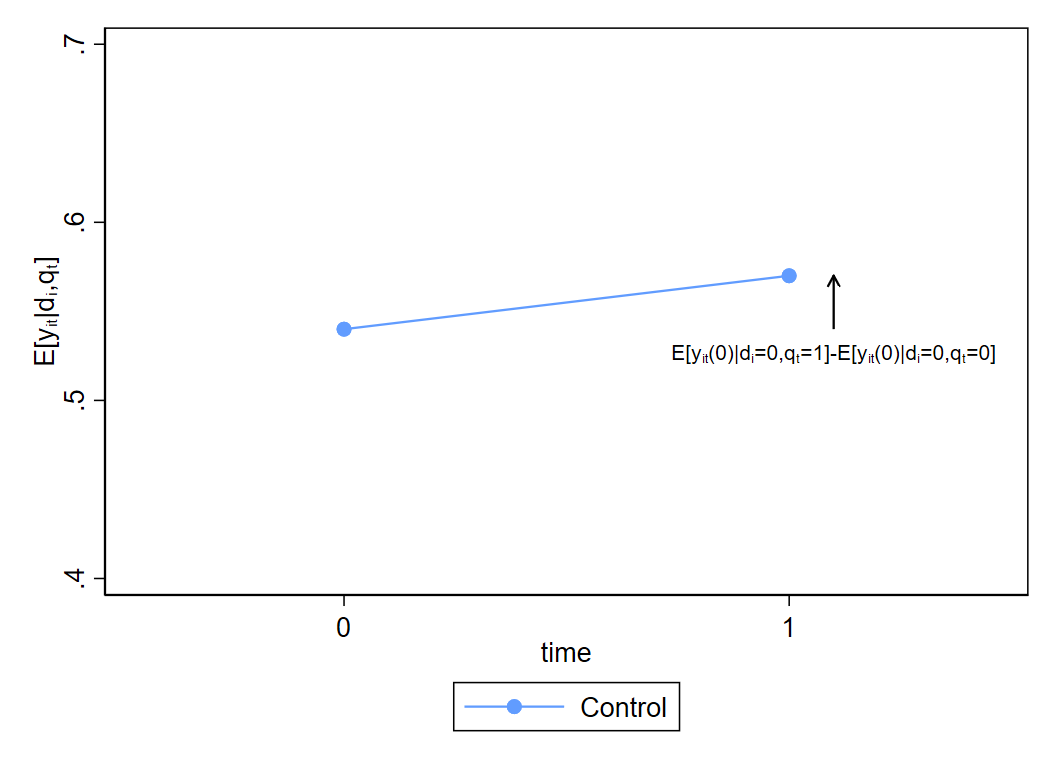
\includegraphics[keepaspectratio]{material/lecture-9/did1.png}}
\end{center}

\subsection{Treatment vs control}\label{treatment-vs-control}

\begin{center}
\pandocbounded{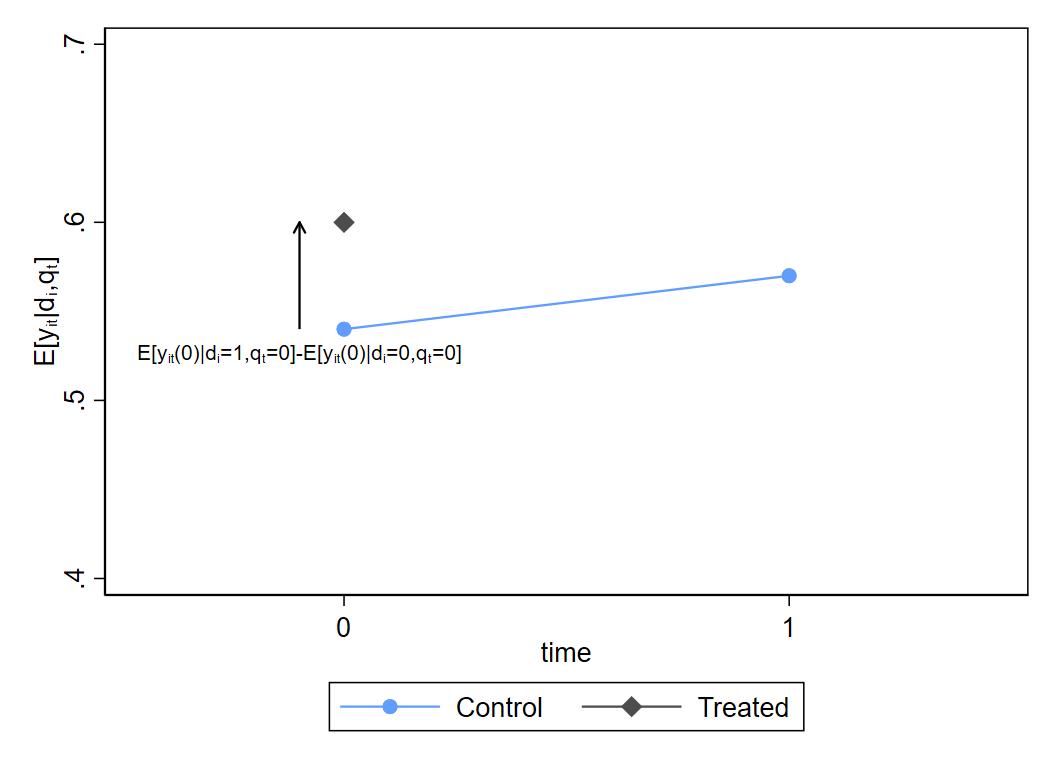
\includegraphics[keepaspectratio]{material/lecture-9/did2.png}}
\end{center}

\subsection{Parallel trends}\label{parallel-trends-1}

\begin{center}
\pandocbounded{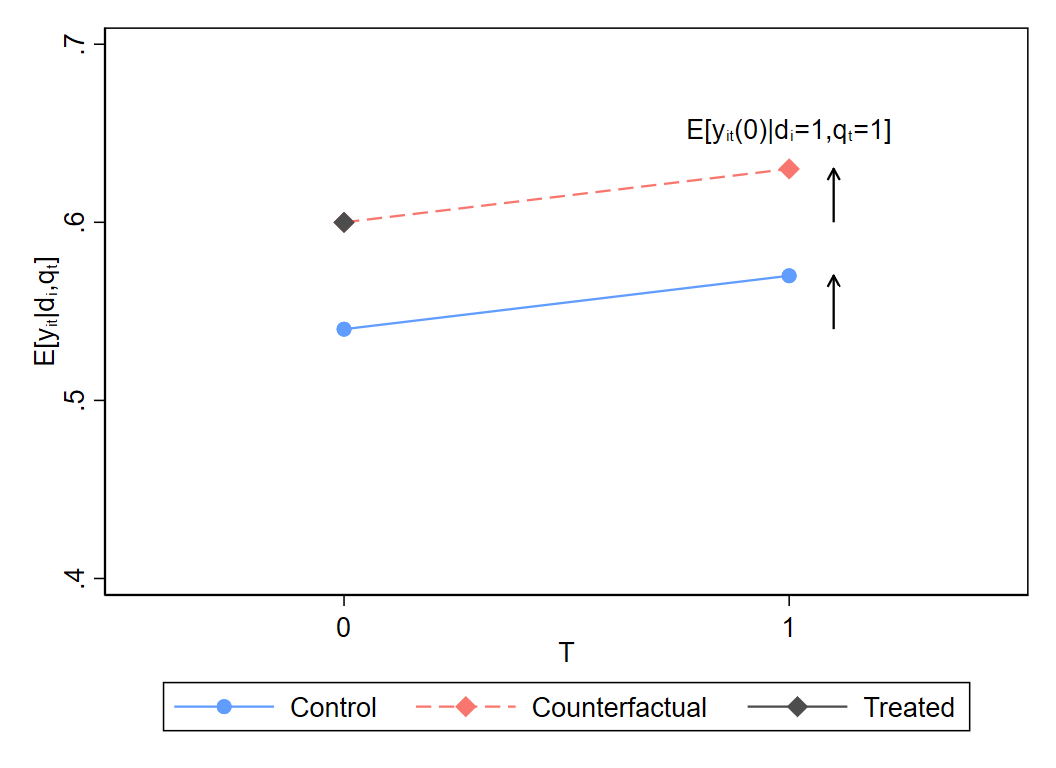
\includegraphics[keepaspectratio]{material/lecture-9/did3.png}}
\end{center}

\subsection{ATT}\label{att}

\begin{center}
\pandocbounded{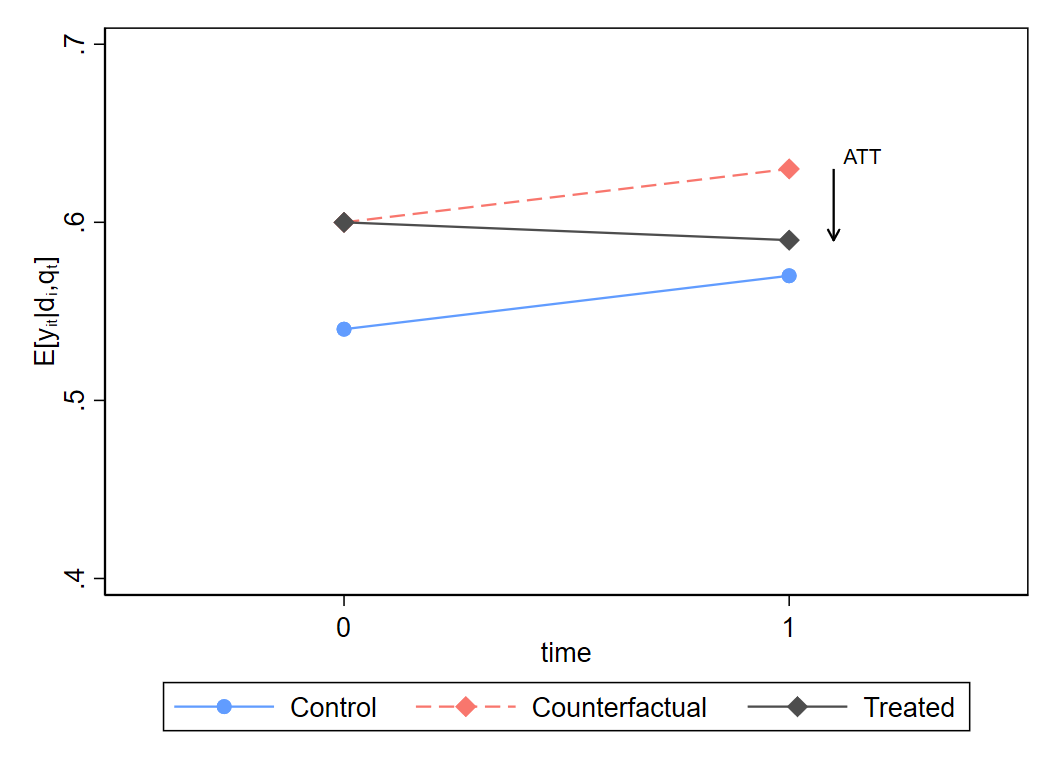
\includegraphics[keepaspectratio]{material/lecture-9/did4.png}}
\end{center}

\section{Linear Model}\label{linear-model}

\subsection{Dummy interaction}\label{dummy-interaction}

We will skip the lengthy approach of \href{lecture-6-multi.qmd}{Lecture
6} and consider the model:

\[
  y_{it} = \alpha + \psi d_i + \delta q_t + \beta d_i\times q_t + \varepsilon_{it}
\]

where, \(d_i\times q_t\) is an interaction of the two dummy variables.

\subsection{CEFs}\label{cefs}

Let's consider the CE of \(y_{it}\) for combination of \(d_i,q_t\)

\begin{enumerate}
\def\labelenumi{\arabic{enumi}.}
\item
  \(E[y_{it}|d_i=0,q_t=0] = \alpha\)
\item
  \(E[y_{it}|d_i=0,q_t=1] = \alpha+\delta\)

  \begin{itemize}
  \item
    \(\Rightarrow \delta = E[y_{it}|d_i=0,q_t=1]-E[y_{it}|d_i=0,q_t=0]\)
  \item
    \(\delta\) captures the mean difference in \(y\) in the control
    group over time.
  \end{itemize}
\item
  \(E[y_{it}|d_i=1,q_t=0] = \alpha+\psi\)

  \begin{itemize}
  \item
    \(\Rightarrow \psi = E[y_{it}|d_i=1,q_t=0]-E[y_{it}|d_i=0,q_t=0]\)
  \item
    \(\psi\) captures the mean difference between treated and control,
    in the pre-period.
  \end{itemize}
\end{enumerate}

\subsection{}\label{section-5}

\begin{enumerate}
\def\labelenumi{\arabic{enumi}.}
\setcounter{enumi}{3}
\item
  \(E[y_{it}|d_i=1,q_t=1] = \alpha + \psi + \delta + \beta\)

  \[
    \begin{aligned}
    \Rightarrow \beta =& \big[\underbrace{E[y_{it}|d_i=1,q_t=1]-E[y_{it}|d_i=0,q_t=1]}_{(\alpha + \psi + \delta + \beta)-(\alpha+\delta)=\beta + \psi}\big] \\
    &-\big[\underbrace{E[y_{it}|d_i=1,q_t=0]-E[y_{it}|d_i=0,q_t=0]}_{(\alpha+\psi)-(\alpha)=\psi}\big]
    \end{aligned}
  \]

  \begin{itemize}
  \item
    \(\beta\) is the DID estimand.
  \item
    \(\beta\) is the ATT under assumptions: (1) parallel trends, (2) no
    anticipation
  \end{itemize}
\end{enumerate}

\subsection{Control group}\label{control-group-1}

\[
  y_{it} = \alpha + \psi d_i + \delta q_t + \beta d_i\times q_t + \varepsilon_{it}
\]

\begin{center}
\pandocbounded{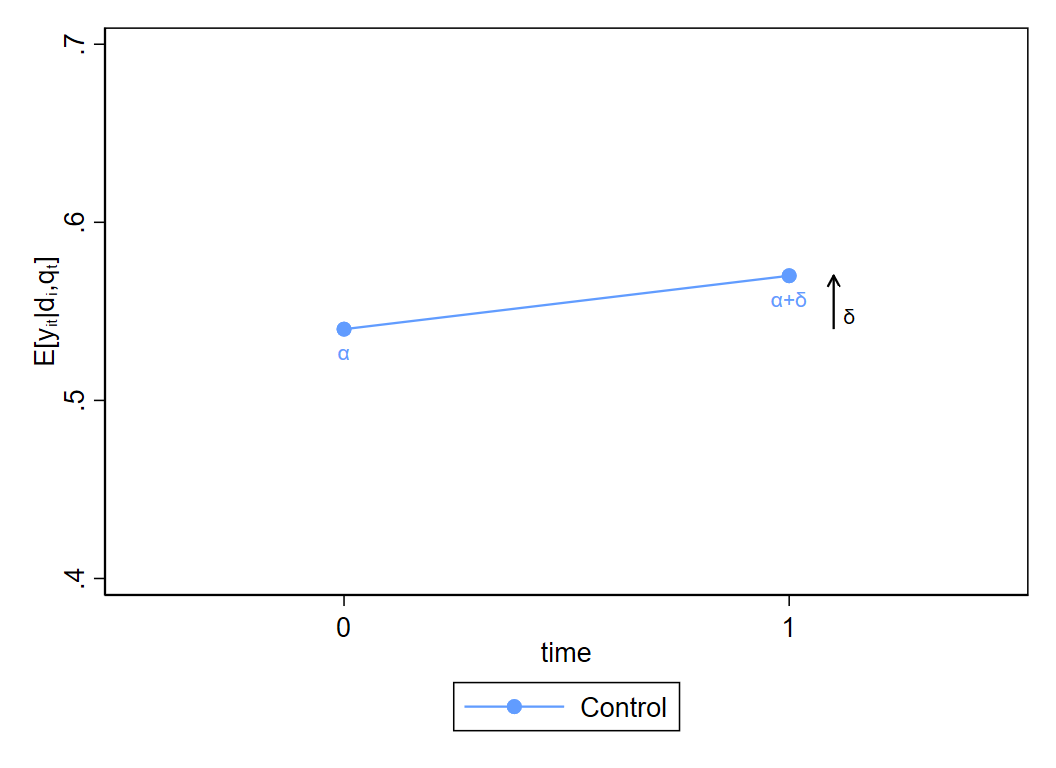
\includegraphics[keepaspectratio]{material/lecture-9/did5.png}}
\end{center}

\subsection{Treatment vs control}\label{treatment-vs-control-1}

\[
  y_{it} = \alpha + \psi d_i + \delta q_t + \beta d_i\times q_t + \varepsilon_{it}
\]

\begin{center}
\pandocbounded{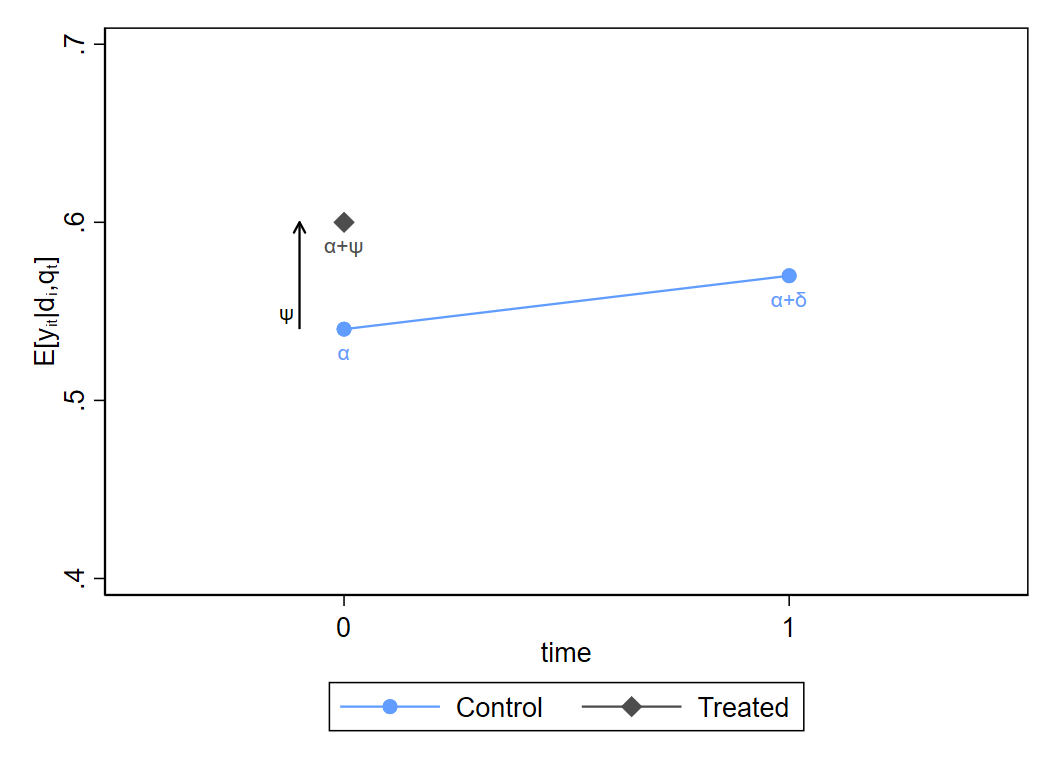
\includegraphics[keepaspectratio]{material/lecture-9/did6.png}}
\end{center}

\subsection{Parallel trends}\label{parallel-trends-2}

\[
  y_{it} = \alpha + \psi d_i + \delta q_t + \beta d_i\times q_t + \varepsilon_{it}
\]

\begin{center}
\pandocbounded{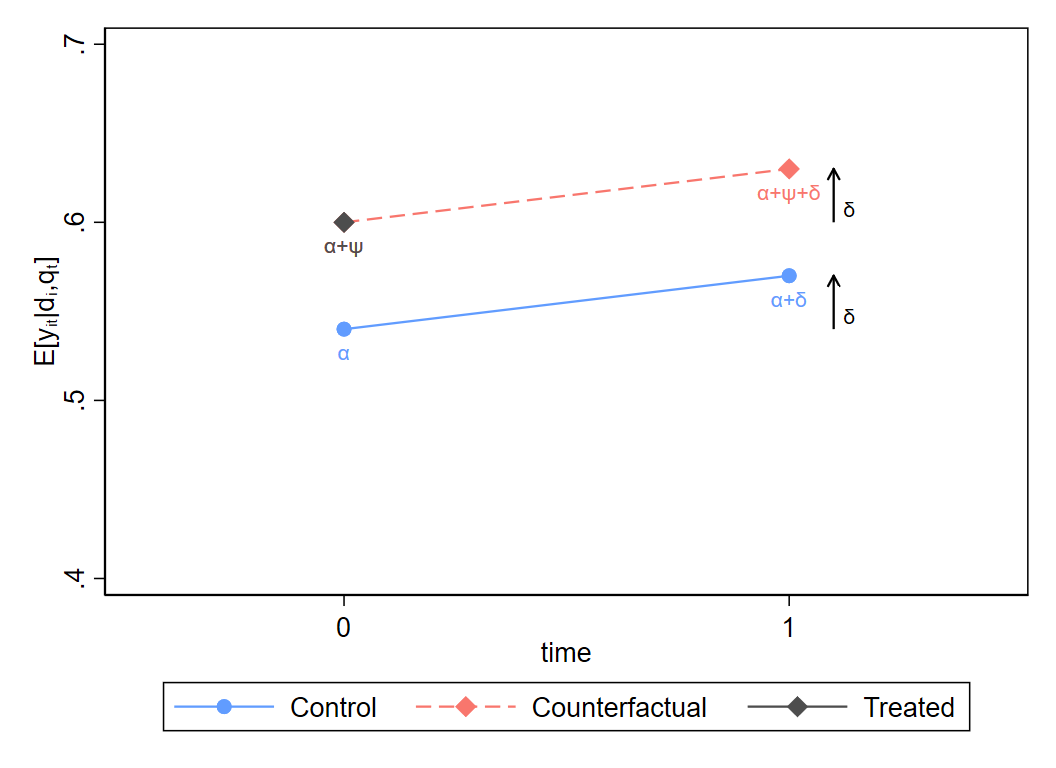
\includegraphics[keepaspectratio]{material/lecture-9/did7.png}}
\end{center}

\subsection{ATT}\label{att-1}

\[
  y_{it} = \alpha + \psi d_i + \delta q_t + \beta d_i\times q_t + \varepsilon_{it}
\]

\begin{center}
\pandocbounded{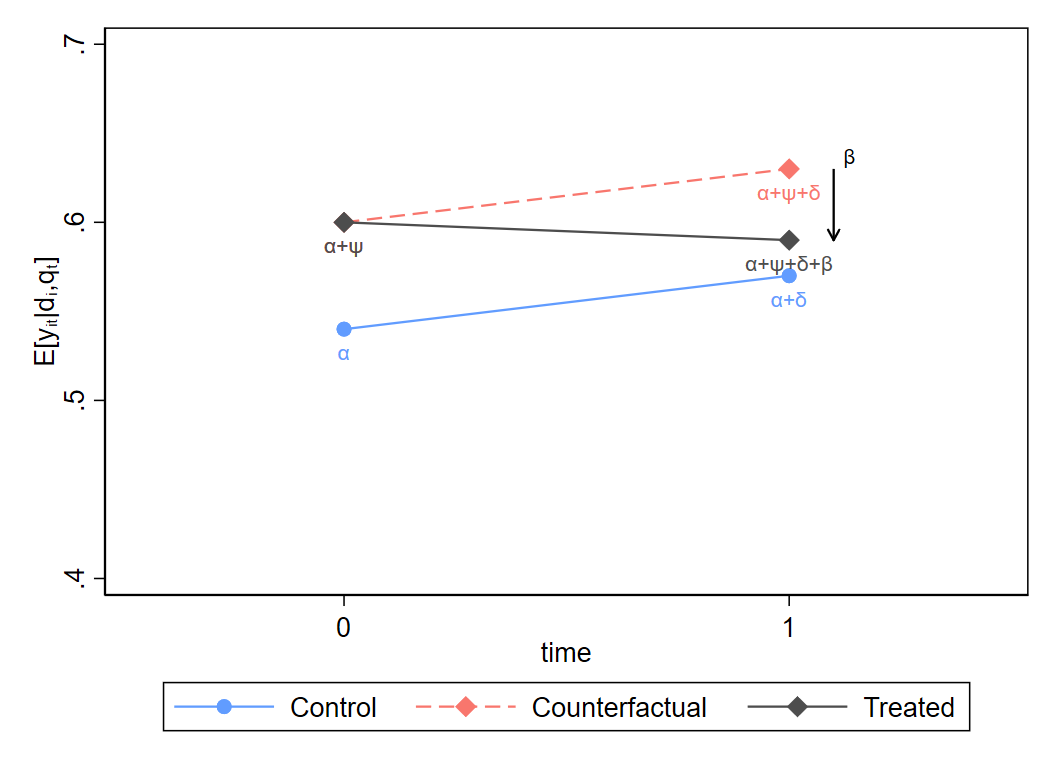
\includegraphics[keepaspectratio]{material/lecture-9/did8.png}}
\end{center}

\subsection{ATT vs ATE}\label{att-vs-ate}

So, under parallel trends and no anticipation:

\[
  y_{it} = \alpha + \psi d_i + \delta q_t + \tau_{att} d_i\times q_t + \varepsilon_{it}
\]

\textbf{Why ATT and not ATE?}

\begin{itemize}
\item
  You need unconfoundedness to learn about the ATE.
\item
  Here we are relying on parallel trends as our identifying assumption.

  \begin{itemize}
  \item
    Doesn't rule out selection into treatment
  \item
    But rather assumes selection is time-invariant
  \end{itemize}
\end{itemize}

\subsection{Covariates}\label{covariates}

What if you add covariates?

\[
  y_{it} = \alpha + \psi d_i + \delta q_t + \tau_{att} d_i\times q_t + \mathbf{x}_{it}\gamma + \upsilon_{it}
\]

\begin{itemize}
\item
  They must be ``good'' controls
\item
  Should improve power (as with RCT)
\item
  Likely correlated with \(d_i\), potentially \(q_t\)
\item
  Unlikely to be correlated with \(d_i\times q_t\)

  \begin{itemize}
  \item
    unless: outcomes of experiment
  \item
    if correlated (i.e.~estimates change a lot after adding controls),
    you should ask why?
  \end{itemize}
\end{itemize}

\section{Example: MW}\label{example-mw}

\subsection{MW debate}\label{mw-debate}

There has been a extended debate in the labour economic literature on
the impact of Minimum Wages:

\begin{itemize}
\item
  Pre-1990's literature:

  \begin{itemize}
  \item
    Mostly supported the idea that an higher minimum wages reduce
    employment.
  \item
    Wellington (1991) \& Brown et al.~(1983): 10\% increase in minimum
    wage reduce teen employment by 1\%.
  \item
    Largely based on time-series evidence (Brown et al., 1982) or
    cross-country studies.
  \end{itemize}
\end{itemize}

\begin{quote}
``Isolating the impacts of labor market institutions is inherently
difficult\ldots{} Identification issues essentially result from the
endogeneity of labor market institutions and the interactions between
them\ldots{} makes it difficult to attribute variations in outcomes to
the institutions themselves, rather than other features of the societies
in which they exist.'' Baetcherman (2012)
\end{quote}

\subsection{Card (1994)}\label{card-1994}

Card and Krueger (1994) is a seminal paper in both the MW and ``natural
experiments'' literatures
(\href{https://davidcard.berkeley.edu/papers/njmin-aer.pdf}{available
online})

\begin{center}
\pandocbounded{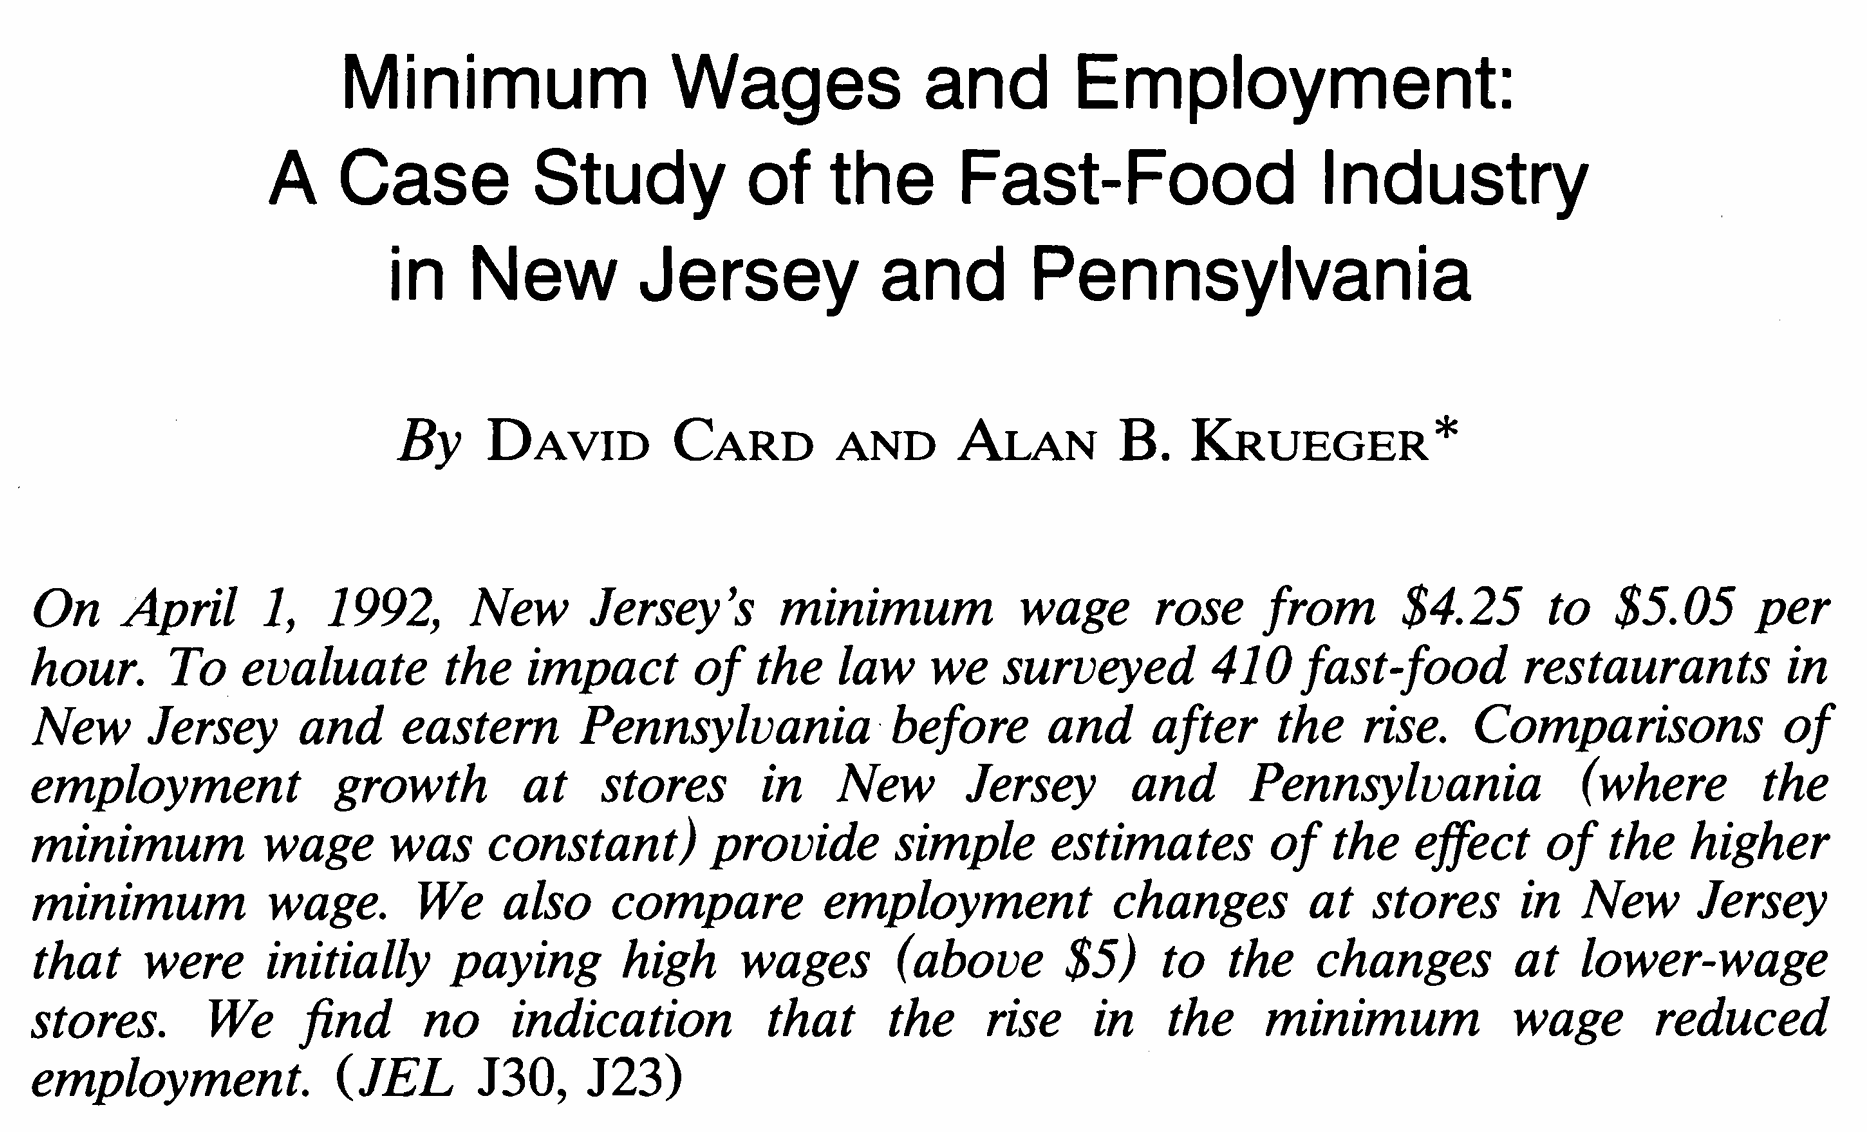
\includegraphics[keepaspectratio]{material/lecture-9/ck1994.png}}
\end{center}

\subsection{}\label{section-6}

Exploit a natural experiment:

\begin{itemize}
\item
  Increase in New Jersey minimum wage from \$4.25 to \$5.05 (19\%),
  April 1992
\item
  Examine the impact on employment at fast food outlets (low wage jobs)
\item
  Use Pennsylvania as a control group in a DiD research design
\item
  \textbf{Results}: Find no evidence of a negative employment effect
\item
  This paper highlights the fact that you can make strong conclusions
  from what is effectively a very simple research design.
\end{itemize}

\subsection{Institution change}\label{institution-change}

This minimum wage change was not unexpected:

\begin{itemize}
\tightlist
\item
  Federal minimum wage is the floor to all state level minimum wages
\item
  Federal increase from \$3.35 \(\rightarrow\) \$3.80 in April 1990
\item
  Federal increase from \$3.80 \(\rightarrow\) \$4.25 in April 1991
\item
  New Jersey choose to increase its own minimum wage to \$5.05 effect
  April 1992, giving it the highest minimum wage in the country.
\item
  Opposed by business leaders, but the opposition lost an appeal (March,
  1992) by a close margin.
\end{itemize}

This last minute appeal and close election do create some uncertainty.

\subsection{Card's setup}\label{cards-setup}

\[
  d_i = \begin{cases} 
  1\quad \text{if "New Jersey"} \\
  0\quad \text{if "Pennsylvania"}
  \end{cases}
\]

\[
  q_t = \begin{cases} 
  1 \quad \text{if}\;t>\text{April 1992} \\
  0 \quad \text{otherwise}
  \end{cases}
\]

\subsection{Data}\label{data-1}

The authors collect their own data using a phone survey of employers:

\begin{figure}[H]

{\centering \pandocbounded{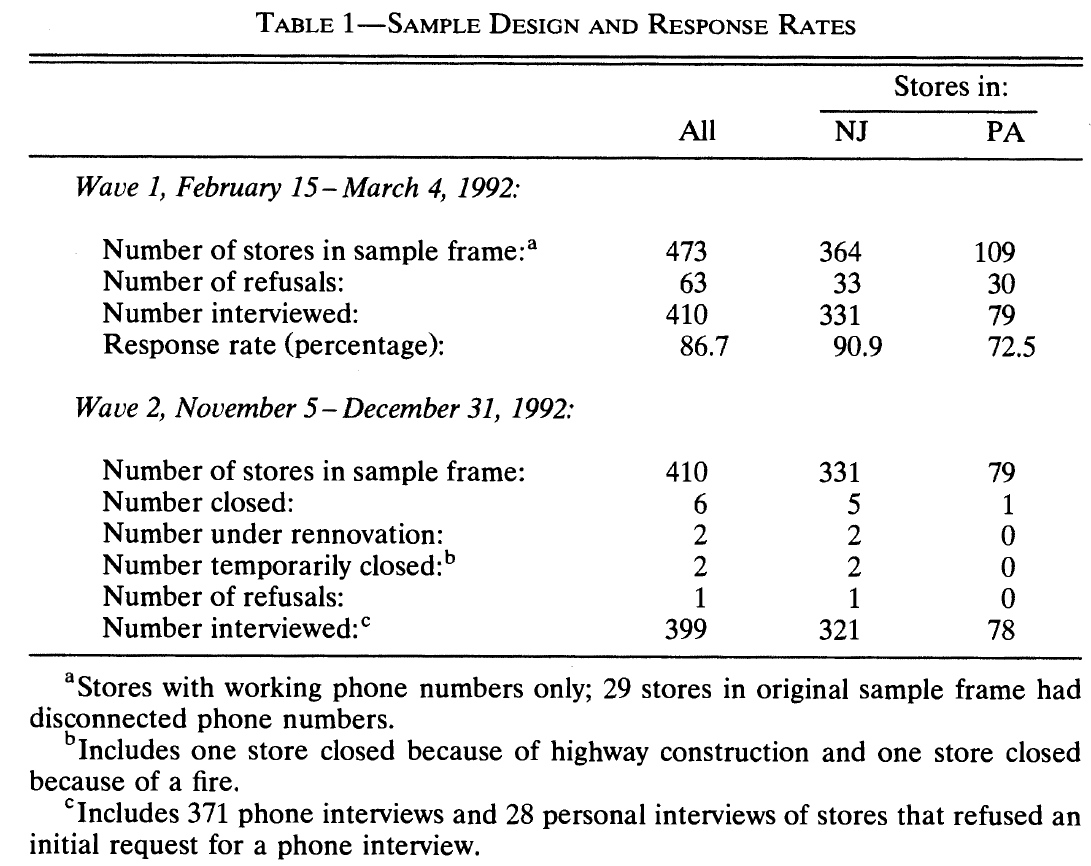
\includegraphics[keepaspectratio]{material/lecture-9/ck1994_table_sample.png}}

}

\caption{p.~774}

\end{figure}%

\subsection{Pre vs post}\label{pre-vs-post}

In the pre-period the states had similar wage distributions

\begin{center}
\pandocbounded{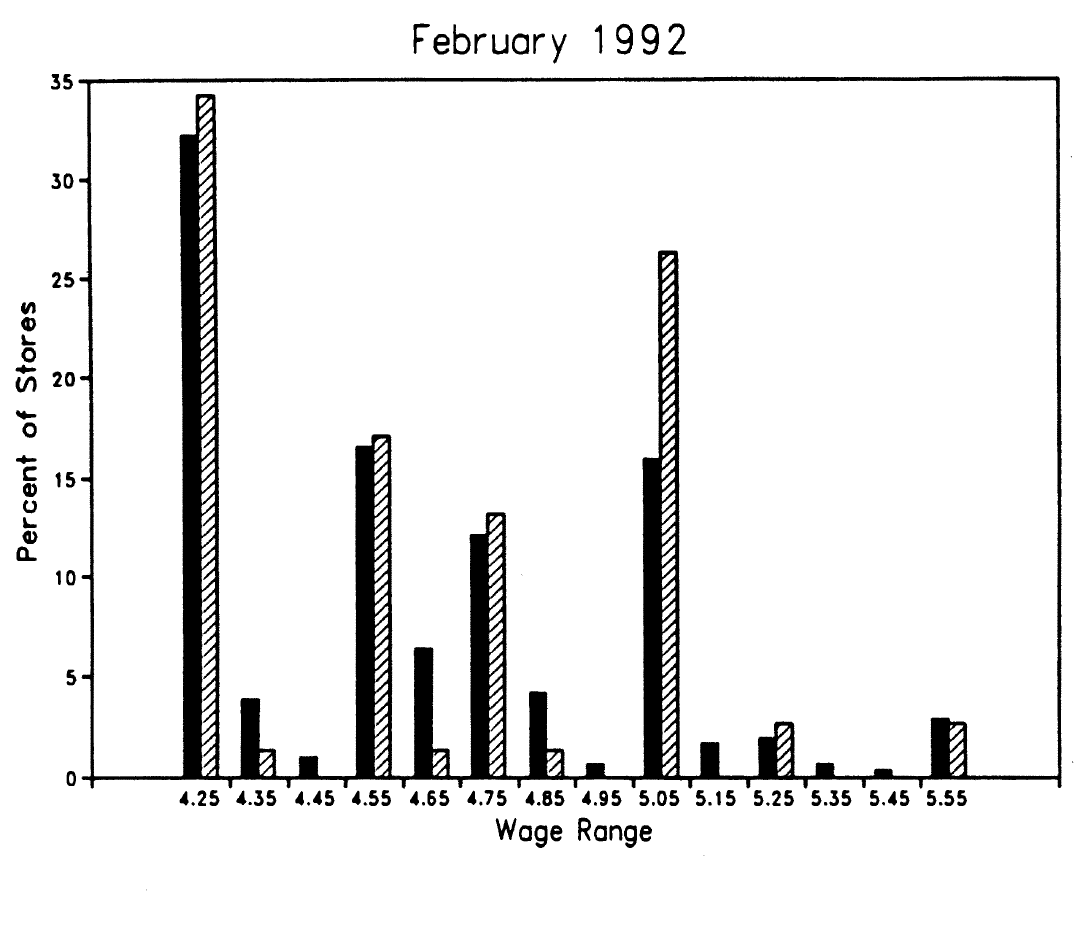
\includegraphics[keepaspectratio]{material/lecture-9/ck1994_wages1.png}}
\end{center}

\begin{figure}[H]

{\centering \pandocbounded{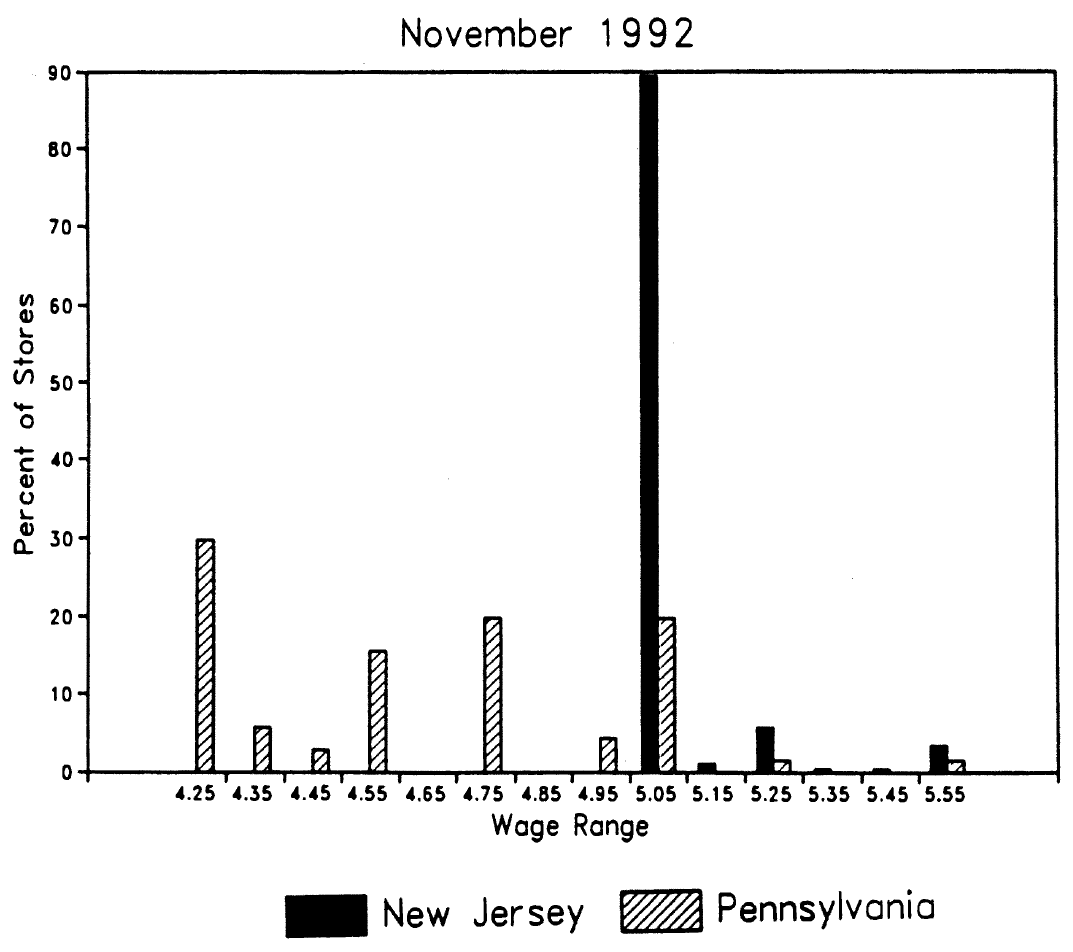
\includegraphics[keepaspectratio]{material/lecture-9/ck1994_wages2.png}}

}

\caption{p.~777}

\end{figure}%

\subsection{DID}\label{did}

No evidence of a negative effect, as competitive models would predict.

\begin{center}
\pandocbounded{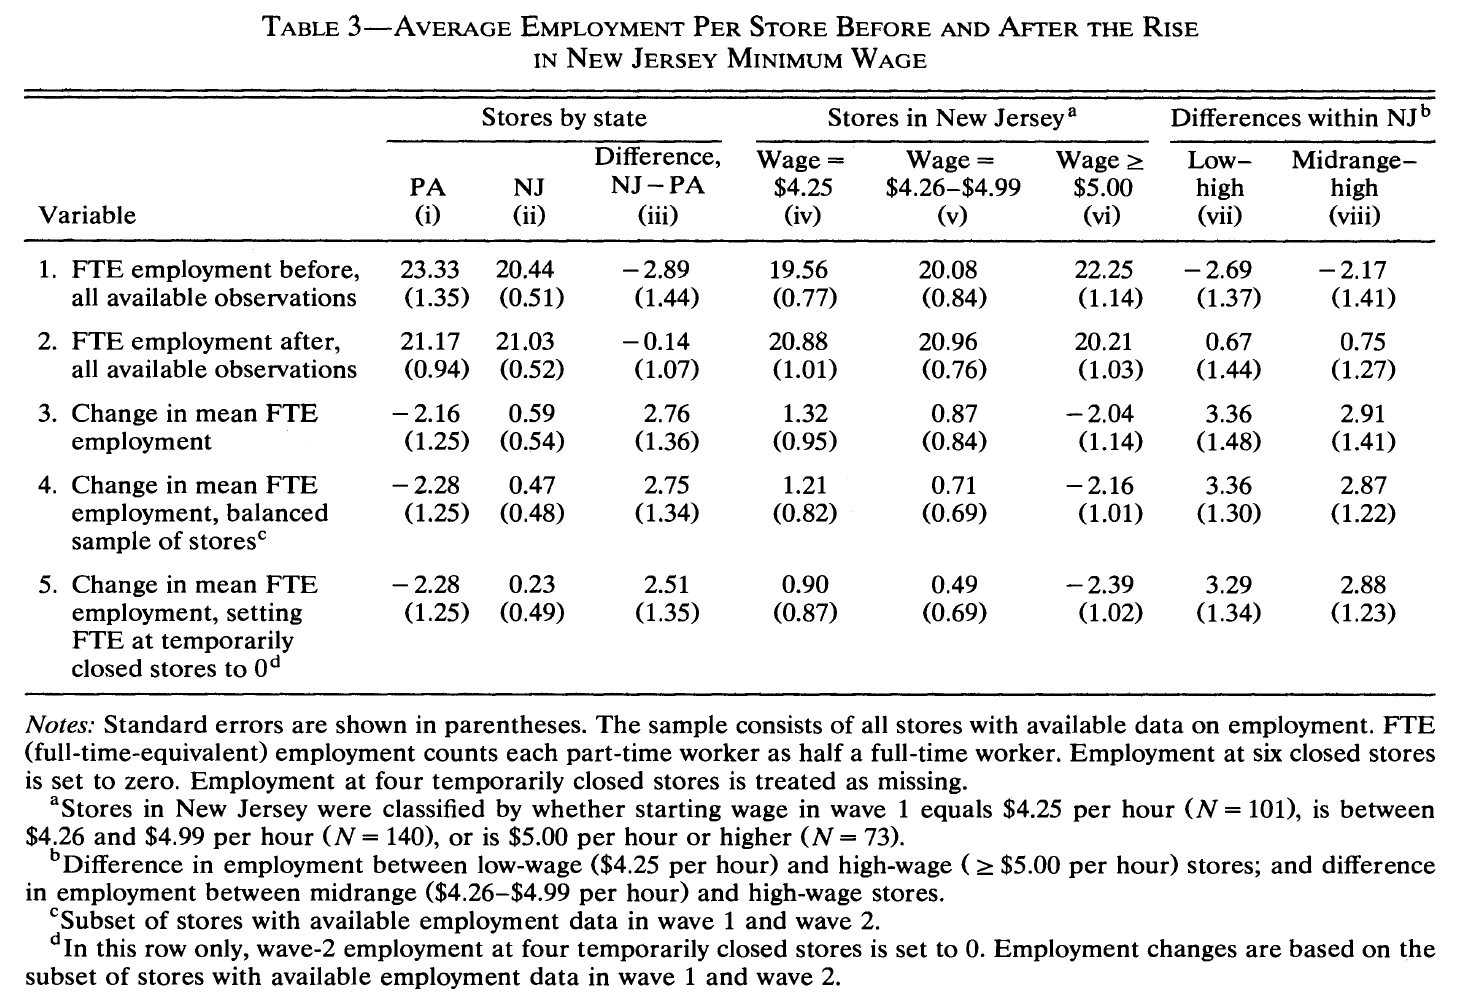
\includegraphics[keepaspectratio]{material/lecture-9/ck1994_table_did.png}}
\end{center}
- If anything, some evidence of small positive effect, as suggested by
monopsonistic models.

\subsection{MW debate}\label{mw-debate-1}

\begin{itemize}
\item
  Card \& Krueger (1994) don't show pre-trends to help persuade you that
  the parallel trends assumption is likely to hold.
\item
  After this paper comes the rebuttal by Neumark \& Wascher (2000, AER),
  followed immediately by a response from Card \& Krueger (2000, AER).
\item
  This is just round 1 of what is a multi-round debate. The discussion
  has now shifted away from state-level minimum wages to the study of
  city-specific policies.
\end{itemize}

\section{Modern Application}\label{modern-application}

\subsection{}\label{section-7}

It was 1 January 2018 and Kathleen Wynne was keen to salvage her
reelection bid for the premiership of Ontario, Canada.

\pandocbounded{
\includegraphics[keepaspectratio]{material/lecture-9/ontario.jpeg}}

\subsection{}\label{section-8}

The governing liberal party announced an unexpected (non-standard)
minimum wage increase of \$2.40 (from \$11.60 to \$14, or 21\%). With a
\$2.25 increase for those under 18 and \$2.10 for liquor servers.

\begin{center}
\pandocbounded{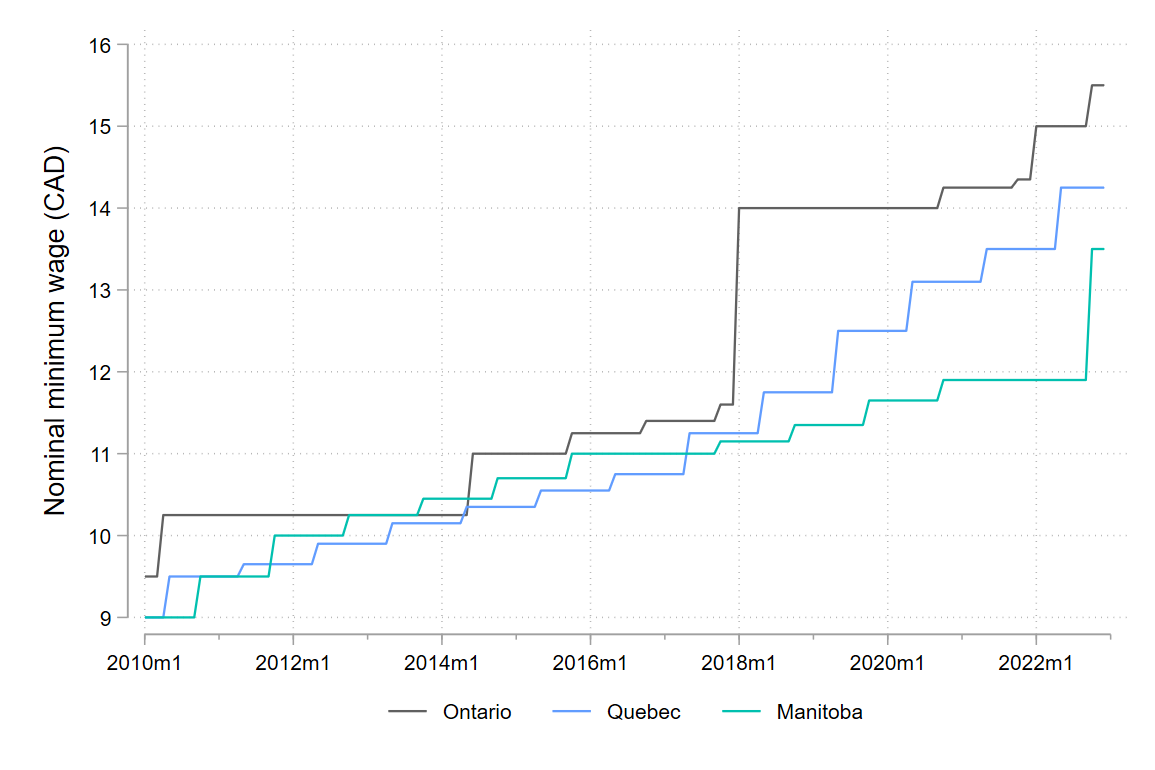
\includegraphics[keepaspectratio]{material/lecture-9/min_wage.png}}
\end{center}

\subsection{Set-up}\label{set-up}

\[
  d_i = \begin{cases} 
  1 \;\text{if "Ontario"}\\
  0 \; \text{if "Quebec" or "Manitoba"}
  \end{cases}
\]

\hfill\break

\[
  q_t = \begin{cases} 
  1\;\text{if}\;t=2018 \\
  0\;\text{if}\;t=2017
  \end{cases}
\]

\subsection{Graphical results}\label{graphical-results}

Here I am plotting the employment rate (employment-population ratio) of
young individuals aged 15-29

\begin{Shaded}
\begin{Highlighting}[]
\KeywordTok{preserve}
\KeywordTok{qui} \KeywordTok{keep} \KeywordTok{if} \FunctionTok{inlist}\NormalTok{(agegrp,1,3)}
\KeywordTok{collapse}\NormalTok{ (}\KeywordTok{mean}\NormalTok{) employ, }\KeywordTok{by}\NormalTok{(province }\FunctionTok{year}\NormalTok{)}
\KeywordTok{twoway}\NormalTok{  (connected employ }\FunctionTok{year} \KeywordTok{if}\NormalTok{ province==6) (connected employ }\FunctionTok{year} \KeywordTok{if}\NormalTok{ province==5, ms(S))  (connected employ }\FunctionTok{year} \KeywordTok{if}\NormalTok{ province==7, ms(D)) }\KeywordTok{if} \FunctionTok{inlist}\NormalTok{(}\FunctionTok{year}\NormalTok{,2017,2018), }\BaseNTok{legend}\NormalTok{(}\KeywordTok{order}\NormalTok{(1 }\StringTok{"Ontario"}\NormalTok{ 2 }\StringTok{"Quebec"}\NormalTok{ 3 }\StringTok{"Manitoba"}\NormalTok{) }\FunctionTok{r}\NormalTok{(1) pos(6)) }\BaseNTok{ytitle}\NormalTok{(Employment rate)  }\KeywordTok{ylabel}\NormalTok{(0.2(.1).8, }\KeywordTok{format}\NormalTok{(\%2.1f)) }\KeywordTok{xlabel}\NormalTok{(2017 2018) xmtick(2016.5(.5)2018.5)}
\KeywordTok{restore}
\end{Highlighting}
\end{Shaded}

\begin{center}
\pandocbounded{\includegraphics[keepaspectratio]{lecture-9-R_files/figure-pdf/unnamed-chunk-9-1.pdf}}
\end{center}

\subsection{Regression}\label{regression}

\begin{Shaded}
\begin{Highlighting}[]
\KeywordTok{gen}\NormalTok{ treat = province==6}
\KeywordTok{gen} \KeywordTok{post}\NormalTok{ = }\FunctionTok{year}\NormalTok{\textgreater{}=2018}
\KeywordTok{gen}\NormalTok{ trtpost = treat*}\KeywordTok{post}

\KeywordTok{gen}\NormalTok{ city = }\FunctionTok{inlist}\NormalTok{(cma,2,4,9)}
\KeywordTok{tab} \FunctionTok{year}\NormalTok{ city}
\KeywordTok{gen}\NormalTok{ female = sex==2}
\end{Highlighting}
\end{Shaded}

Quebec as control group

\begin{Shaded}
\begin{Highlighting}[]
\KeywordTok{est} \KeywordTok{clear}
\NormalTok{eststo: }\KeywordTok{qui} \KeywordTok{reg}\NormalTok{ employ treat }\KeywordTok{post}\NormalTok{ trtpost }\KeywordTok{if} \FunctionTok{inlist}\NormalTok{(province,5,6) \& }\FunctionTok{inlist}\NormalTok{(}\FunctionTok{year}\NormalTok{,2017,2018) \& }\FunctionTok{inlist}\NormalTok{(agegrp,1,3), }\FunctionTok{r}
\NormalTok{eststo: }\KeywordTok{qui} \KeywordTok{reg}\NormalTok{ employ treat }\KeywordTok{post}\NormalTok{ trtpost i.}\FunctionTok{month} \KeywordTok{if} \FunctionTok{inlist}\NormalTok{(province,5,6) \& }\FunctionTok{inlist}\NormalTok{(}\FunctionTok{year}\NormalTok{,2017,2018) \& }\FunctionTok{inlist}\NormalTok{(agegrp,1,3), }\FunctionTok{r}
\NormalTok{eststo: }\KeywordTok{qui} \KeywordTok{reg}\NormalTok{ employ treat }\KeywordTok{post}\NormalTok{ trtpost i.}\FunctionTok{month}\NormalTok{ female city i.efamtype i.edugrp }\KeywordTok{if} \FunctionTok{inlist}\NormalTok{(province,5,6) \& }\FunctionTok{inlist}\NormalTok{(}\FunctionTok{year}\NormalTok{,2017,2018) \& }\FunctionTok{inlist}\NormalTok{(agegrp,1,3), }\FunctionTok{r}

\NormalTok{esttab, }\KeywordTok{replace}\NormalTok{ se }\KeywordTok{star}\NormalTok{(* 0.1 ** 0.05 *** 0.01) }\KeywordTok{keep}\NormalTok{(}\DataTypeTok{\_cons}\NormalTok{ treat }\KeywordTok{post}\NormalTok{ trtpost) }\KeywordTok{order}\NormalTok{(}\DataTypeTok{\_cons}\NormalTok{ treat }\KeywordTok{post}\NormalTok{ trtpost) indicate(}\StringTok{"Month FE = 2.month"} \StringTok{"Covariates = 2.efamtype"}\NormalTok{) }
\end{Highlighting}
\end{Shaded}

\begin{verbatim}
(est1 stored)

(est2 stored)

(est3 stored)


------------------------------------------------------------
                      (1)             (2)             (3)   
                   employ          employ          employ   
------------------------------------------------------------
_cons               0.656***        0.621***        0.620***
                (0.00286)       (0.00509)       (0.00587)   

treat             -0.0503***      -0.0501***      -0.0130***
                (0.00364)       (0.00364)       (0.00329)   

post               0.0354***       0.0354***       0.0255***
                (0.00401)       (0.00401)       (0.00359)   

trtpost           -0.0253***      -0.0251***      -0.0245***
                (0.00513)       (0.00512)       (0.00459)   

Month FE               No             Yes             Yes   

Covariates             No              No             Yes   
------------------------------------------------------------
N                  147798          147798          147798   
------------------------------------------------------------
Standard errors in parentheses
* p<0.1, ** p<0.05, *** p<0.01
\end{verbatim}

\subsection{}\label{section-9}

Manitoba as control group

\begin{Shaded}
\begin{Highlighting}[]
\KeywordTok{est} \KeywordTok{clear}
\NormalTok{eststo: }\KeywordTok{qui} \KeywordTok{reg}\NormalTok{ employ treat }\KeywordTok{post}\NormalTok{ trtpost }\KeywordTok{if} \FunctionTok{inlist}\NormalTok{(province,7,6) \& }\FunctionTok{inlist}\NormalTok{(}\FunctionTok{year}\NormalTok{,2017,2018) \& }\FunctionTok{inlist}\NormalTok{(agegrp,1,3), }\FunctionTok{r}
\NormalTok{eststo: }\KeywordTok{qui} \KeywordTok{reg}\NormalTok{ employ treat }\KeywordTok{post}\NormalTok{ trtpost i.}\FunctionTok{month} \KeywordTok{if} \FunctionTok{inlist}\NormalTok{(province,7,6) \& }\FunctionTok{inlist}\NormalTok{(}\FunctionTok{year}\NormalTok{,2017,2018) \& }\FunctionTok{inlist}\NormalTok{(agegrp,1,3), }\FunctionTok{r}
\NormalTok{eststo: }\KeywordTok{qui} \KeywordTok{reg}\NormalTok{ employ treat }\KeywordTok{post}\NormalTok{ trtpost i.}\FunctionTok{month}\NormalTok{ female city i.efamtype i.edugrp }\KeywordTok{if} \FunctionTok{inlist}\NormalTok{(province,7,6) \& }\FunctionTok{inlist}\NormalTok{(}\FunctionTok{year}\NormalTok{,2017,2018) \& }\FunctionTok{inlist}\NormalTok{(agegrp,1,3), }\FunctionTok{r}

\NormalTok{esttab, }\KeywordTok{replace}\NormalTok{ se }\KeywordTok{star}\NormalTok{(* 0.1 ** 0.05 *** 0.01) }\KeywordTok{keep}\NormalTok{(}\DataTypeTok{\_cons}\NormalTok{ treat }\KeywordTok{post}\NormalTok{ trtpost) }\KeywordTok{order}\NormalTok{(}\DataTypeTok{\_cons}\NormalTok{ treat }\KeywordTok{post}\NormalTok{ trtpost) indicate(}\StringTok{"Month FE = 2.month"} \StringTok{"Covariates = 2.efamtype"}\NormalTok{) }
\end{Highlighting}
\end{Shaded}

\begin{verbatim}
(est1 stored)

(est2 stored)

(est3 stored)


------------------------------------------------------------
                      (1)             (2)             (3)   
                   employ          employ          employ   
------------------------------------------------------------
_cons               0.603***        0.568***        0.591***
                (0.00358)       (0.00577)       (0.00637)   

treat             0.00262         0.00369          0.0264***
                (0.00423)       (0.00423)       (0.00381)   

post             -0.00220       -0.000755          0.0133***
                (0.00517)       (0.00516)       (0.00458)   

trtpost            0.0123**        0.0111*        -0.0125** 
                (0.00608)       (0.00607)       (0.00540)   

Month FE               No             Yes             Yes   

Covariates             No              No             Yes   
------------------------------------------------------------
N                  129206          129206          129206   
------------------------------------------------------------
Standard errors in parentheses
* p<0.1, ** p<0.05, *** p<0.01
\end{verbatim}

\subsection{}\label{section-10}

Manitoba \& Quebec as pooled control group

\begin{Shaded}
\begin{Highlighting}[]
\KeywordTok{est} \KeywordTok{clear}
\NormalTok{eststo: }\KeywordTok{reg}\NormalTok{ employ treat }\KeywordTok{post}\NormalTok{ trtpost }\KeywordTok{if} \FunctionTok{inlist}\NormalTok{(province,7,6,5) \& }\FunctionTok{inlist}\NormalTok{(}\FunctionTok{year}\NormalTok{,2017,2018) \& }\FunctionTok{inlist}\NormalTok{(agegrp,1,3), }\FunctionTok{r}
\NormalTok{eststo: }\KeywordTok{reg}\NormalTok{ employ treat }\KeywordTok{post}\NormalTok{ trtpost i.}\FunctionTok{month} \KeywordTok{if} \FunctionTok{inlist}\NormalTok{(province,7,6,5) \& }\FunctionTok{inlist}\NormalTok{(}\FunctionTok{year}\NormalTok{,2017,2018) \& }\FunctionTok{inlist}\NormalTok{(agegrp,1,3), }\FunctionTok{r}
\NormalTok{eststo: }\KeywordTok{reg}\NormalTok{ employ treat }\KeywordTok{post}\NormalTok{ trtpost i.}\FunctionTok{month}\NormalTok{ female city i.efamtype i.edugrp }\KeywordTok{if} \FunctionTok{inlist}\NormalTok{(province,7,6,5) \& }\FunctionTok{inlist}\NormalTok{(}\FunctionTok{year}\NormalTok{,2017,2018) \& }\FunctionTok{inlist}\NormalTok{(agegrp,1,3), }\FunctionTok{r}

\NormalTok{esttab, }\KeywordTok{replace}\NormalTok{ se }\KeywordTok{star}\NormalTok{(* 0.1 ** 0.05 *** 0.01) }\KeywordTok{keep}\NormalTok{(}\DataTypeTok{\_cons}\NormalTok{ treat }\KeywordTok{post}\NormalTok{ trtpost) }\KeywordTok{order}\NormalTok{(}\DataTypeTok{\_cons}\NormalTok{ treat }\KeywordTok{post}\NormalTok{ trtpost) indicate(}\StringTok{"Month FE = 2.month"} \StringTok{"Covariates = 2.efamtype"}\NormalTok{) }
\end{Highlighting}
\end{Shaded}

\begin{verbatim}
Linear regression                               Number of obs     =    183,723
                                                F(3, 183719)      =      96.69
                                                Prob > F          =     0.0000
                                                R-squared         =     0.0016
                                                Root MSE          =     .48308

------------------------------------------------------------------------------
             |               Robust
      employ | Coefficient  std. err.      t    P>|t|     [95% conf. interval]
-------------+----------------------------------------------------------------
       treat |  -.0289138   .0031789    -9.10   0.000    -.0351444   -.0226832
        post |   .0214282   .0031812     6.74   0.000     .0151931    .0276634
     trtpost |   -.011338   .0045072    -2.52   0.012     -.020172    -.002504
       _cons |   .6345375   .0022417   283.06   0.000     .6301437    .6389312
------------------------------------------------------------------------------
(est1 stored)


Linear regression                               Number of obs     =    183,723
                                                F(14, 183708)     =      73.85
                                                Prob > F          =     0.0000
                                                R-squared         =     0.0055
                                                Root MSE          =     .48215

------------------------------------------------------------------------------
             |               Robust
      employ | Coefficient  std. err.      t    P>|t|     [95% conf. interval]
-------------+----------------------------------------------------------------
       treat |  -.0283528   .0031728    -8.94   0.000    -.0345713   -.0221343
        post |    .022031    .003176     6.94   0.000     .0158061    .0282559
     trtpost |   -.011701   .0044989    -2.60   0.009    -.0205188   -.0028833
             |
       month |
          2  |  -.0039448   .0055821    -0.71   0.480    -.0148857    .0069961
          3  |   .0041902    .005569     0.75   0.452    -.0067249    .0151053
          4  |   .0135607   .0055468     2.44   0.014     .0026892    .0244322
          5  |   .0417467   .0055054     7.58   0.000     .0309562    .0525371
          6  |   .0624812    .005489    11.38   0.000     .0517229    .0732395
          7  |   .0960176   .0054465    17.63   0.000     .0853425    .1066927
          8  |   .0819951   .0054726    14.98   0.000     .0712689    .0927213
          9  |   .0313737   .0055689     5.63   0.000     .0204587    .0422887
         10  |   .0312333   .0055821     5.60   0.000     .0202926    .0421741
         11  |   .0331757   .0055816     5.94   0.000     .0222359    .0441155
         12  |   .0332626   .0055751     5.97   0.000     .0223356    .0441896
             |
       _cons |   .5988005   .0043998   136.10   0.000      .590177    .6074239
------------------------------------------------------------------------------
(est2 stored)


Linear regression                               Number of obs     =    183,723
                                                F(35, 183687)     =    2168.43
                                                Prob > F          =     0.0000
                                                R-squared         =     0.2041
                                                Root MSE          =     .43135

------------------------------------------------------------------------------
             |               Robust
      employ | Coefficient  std. err.      t    P>|t|     [95% conf. interval]
-------------+----------------------------------------------------------------
       treat |   .0027813   .0028482     0.98   0.329    -.0028011    .0083638
        post |   .0209641   .0028296     7.41   0.000     .0154182      .02651
     trtpost |  -.0201467   .0040256    -5.00   0.000    -.0280368   -.0122567
             |
       month |
          2  |  -.0030424   .0049738    -0.61   0.541    -.0127909    .0067062
          3  |    .002576   .0049716     0.52   0.604    -.0071682    .0123202
          4  |   .0099528   .0049456     2.01   0.044     .0002596     .019646
          5  |   .0363644   .0049193     7.39   0.000     .0267227     .046006
          6  |   .0564715   .0048925    11.54   0.000     .0468824    .0660607
          7  |   .0955921   .0049127    19.46   0.000     .0859633    .1052209
          8  |   .0803885   .0049315    16.30   0.000     .0707228    .0900541
          9  |   .0242947   .0049648     4.89   0.000     .0145637    .0340257
         10  |   .0240242   .0049863     4.82   0.000     .0142511    .0337974
         11  |   .0247597   .0049812     4.97   0.000     .0149966    .0345227
         12  |   .0249825   .0049898     5.01   0.000     .0152026    .0347624
             |
      female |   .0011349   .0020581     0.55   0.581    -.0028989    .0051688
        city |  -.0915812   .0026874   -34.08   0.000    -.0968484    -.086314
             |
    efamtype |
2. Husban..  |   .1234256   .0030051    41.07   0.000     .1175356    .1293156
3. Husban..  |  -.1059147   .0035046   -30.22   0.000    -.1127837   -.0990456
4. Husban..  |  -.0697179   .0052919   -13.17   0.000    -.0800899   -.0593459
5. Husban..  |  -.1973463    .007925   -24.90   0.000    -.2128791   -.1818135
6. Husban..  |  -.3402987   .0052245   -65.14   0.000    -.3505385   -.3300588
7. Husban..  |  -.0989178   .0108843    -9.09   0.000    -.1202509   -.0775848
8. Husban..  |  -.1388252   .0086216   -16.10   0.000    -.1557234    -.121927
9. Husban..  |   -.253424   .0082304   -30.79   0.000    -.2695554   -.2372925
10. Husba..  |  -.1383649   .0137732   -10.05   0.000    -.1653601   -.1113697
11. Husba..  |   -.298213   .0098215   -30.36   0.000    -.3174628   -.2789632
12. Husba..  |  -.5369095   .0070836   -75.80   0.000    -.5507931   -.5230259
13. Husba..  |  -.2299046   .0188145   -12.22   0.000    -.2667805   -.1930287
14. Singl..  |  -.1895023    .005002   -37.89   0.000    -.1993061   -.1796986
15. Husba..  |  -.1081707   .0078053   -13.86   0.000     -.123469   -.0928724
16. Singl..  |    -.48931   .0062603   -78.16   0.000    -.5015801   -.4770399
17. Singl..  |  -.2105714   .0150241   -14.02   0.000    -.2400183   -.1811245
18. Other..  |  -.0703932   .0044592   -15.79   0.000    -.0791332   -.0616533
             |
      edugrp |
2. Some s..  |   .2051594   .0024487    83.78   0.000     .2003601    .2099588
3. Univer..  |   .2658294   .0029201    91.04   0.000     .2601061    .2715526
             |
       _cons |   .6028886   .0050573   119.21   0.000     .5929764    .6128008
------------------------------------------------------------------------------
(est3 stored)


------------------------------------------------------------
                      (1)             (2)             (3)   
                   employ          employ          employ   
------------------------------------------------------------
_cons               0.635***        0.599***        0.603***
                (0.00224)       (0.00440)       (0.00506)   

treat             -0.0289***      -0.0284***      0.00278   
                (0.00318)       (0.00317)       (0.00285)   

post               0.0214***       0.0220***       0.0210***
                (0.00318)       (0.00318)       (0.00283)   

trtpost           -0.0113**       -0.0117***      -0.0201***
                (0.00451)       (0.00450)       (0.00403)   

Month FE               No             Yes             Yes   

Covariates             No              No             Yes   
------------------------------------------------------------
N                  183723          183723          183723   
------------------------------------------------------------
Standard errors in parentheses
* p<0.1, ** p<0.05, *** p<0.01
\end{verbatim}

\section{Multi-period DID}\label{multi-period-did}

\subsection{2 periods}\label{periods}

With only 2 periods of data (pre- and post-treatment)

\begin{itemize}
\item
  can't provide evidence that parallel trends holds \textbf{in
  pre-period}
\item
  can't provide evidence that there was no pre-emptive response to the
  policy/treatment
\item
  can only show the immediate impact on the outcome

  \begin{itemize}
  \tightlist
  \item
    may under- or over-estimate medium-term impact
  \end{itemize}
\end{itemize}

\subsection{Multiple pre-periods}\label{multiple-pre-periods}

With more pre-treatment data, you can ``eye-ball'' the treatment and
control for evidence of parallel trends and anticipatory responses.

\begin{center}
\pandocbounded{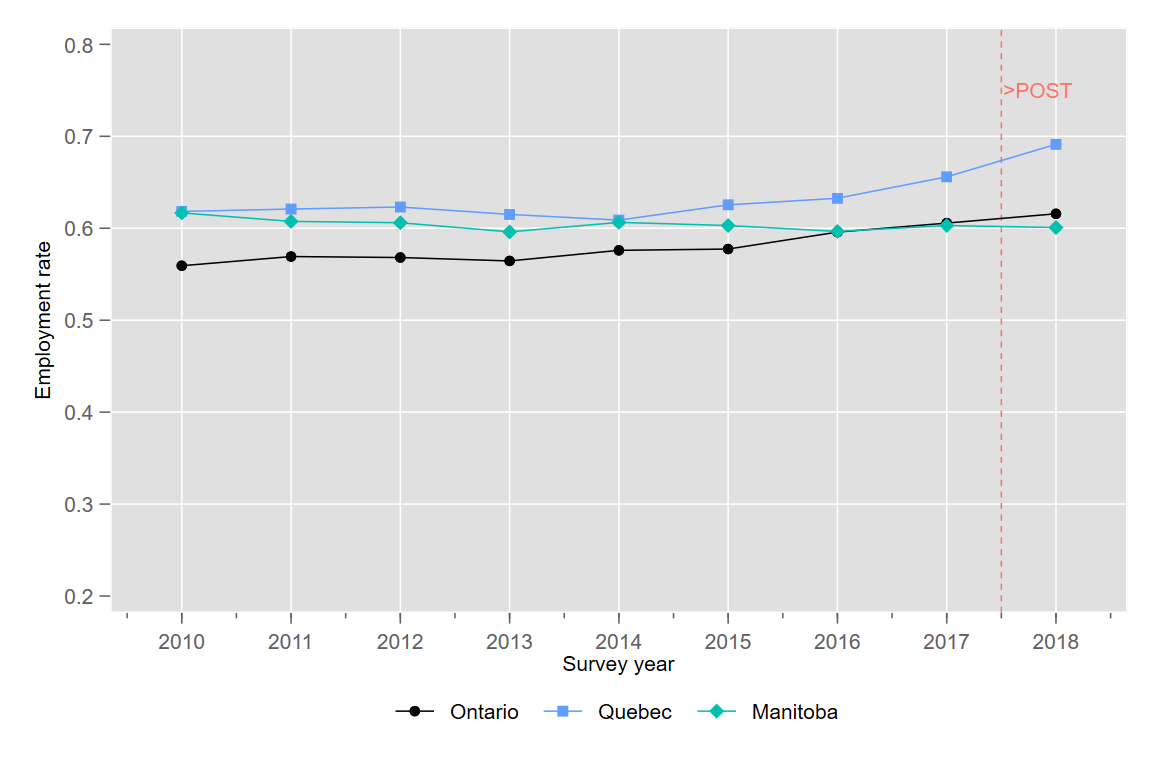
\includegraphics[keepaspectratio]{material/lecture-9/ontario2.png}}
\end{center}

Reviewing the pre-preiod it looks like something may have happened in
Manitoba.

\subsection{Multiple post-periods}\label{multiple-post-periods}

With more post-treatment data, we can ``eye-ball'' whether the
divergence was a once-off phenomenon.

\begin{center}
\pandocbounded{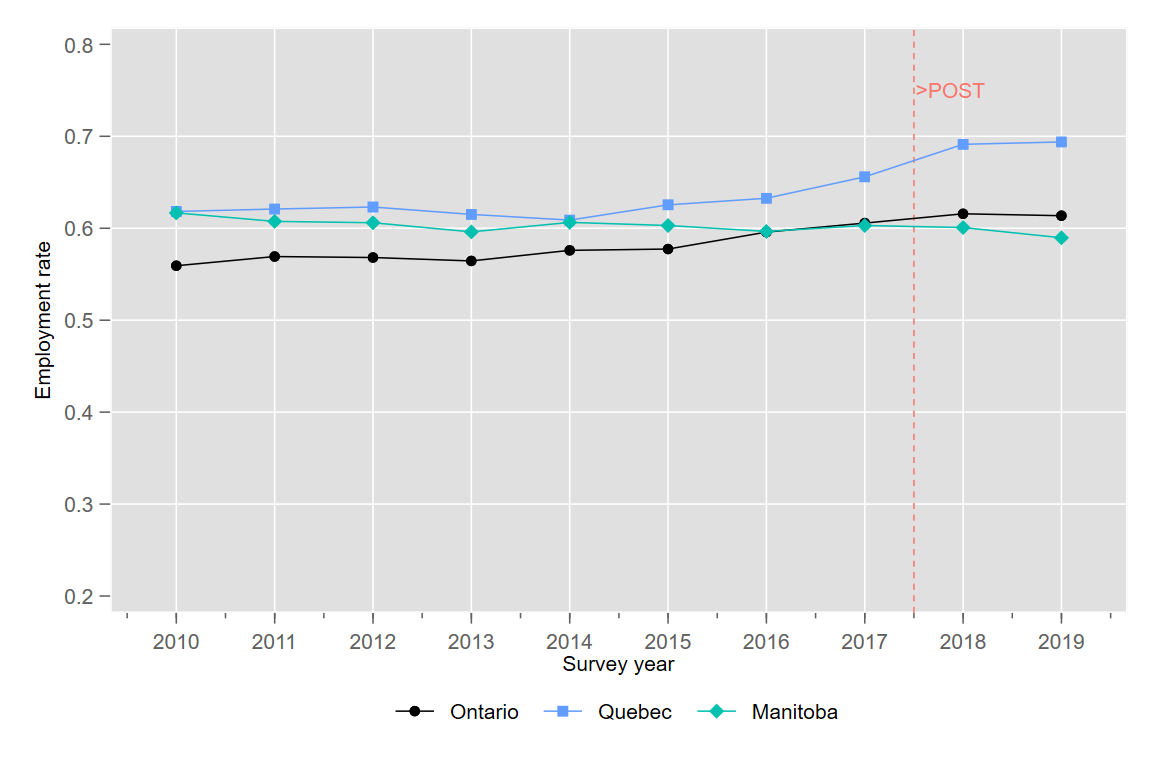
\includegraphics[keepaspectratio]{material/lecture-9/ontario3.png}}
\end{center}

\subsection{2-period model}\label{period-model}

You can estimate the same 2-period model with multiple periods of data:

\[
  y_{it} = \alpha + \psi d_i + \delta q_t + \beta d_i\times q_t + \varepsilon_{it}
\]

\textbf{However,}

\begin{itemize}
\item
  the model ignores potential heterogeneity
\item
  what if the ATT is different in each post-treatment period?
\item
  is \(\beta\) then an average of these post-treatment ATTs?
\end{itemize}

\textbf{This is now a large literature on the complexities of DID
models!} Which we won't get into.

\subsection{}\label{section-11}

In order to write down a more flexible model, we need a richer notation.

\begin{itemize}
\item
  Recall:

  \[
    d_i = \mathbf{1}\{\text{treated}\}\qquad \text{and}\qquad q_t = \mathbf{1}\{t>t_0\}
  \]
\item
  In place of \(q_t\) - which identifies the \emph{whole} post-period -
  we want a variable captures each period relative to the post period.

  \begin{itemize}
  \tightlist
  \item
    e.g.~if treatment is start of 2018 then 2018 is the first year of
    treatment, 2019 is the second
  \end{itemize}
\end{itemize}

\subsection{Option 1: Event-time}\label{option-1-event-time}

Define a measure of time, which captures time since the event:

\[
  s = t-t_0
\]

For example, \(t_0 = 2018\)

\begin{itemize}
\item
  \(t=2018\Rightarrow s = 0\); i.e.~first year of treatment
\item
  \(t=2017\Rightarrow s = -1\); i.e.~year preceeding treatment
\item
  \(t=2019\Rightarrow s = +1\); i.e.~second year since treatment
\end{itemize}

\begin{tcolorbox}[enhanced jigsaw, opacitybacktitle=0.6, colbacktitle=quarto-callout-note-color!10!white, rightrule=.15mm, colframe=quarto-callout-note-color-frame, bottomtitle=1mm, breakable, leftrule=.75mm, colback=white, toprule=.15mm, toptitle=1mm, left=2mm, title=\textcolor{quarto-callout-note-color}{\faInfo}\hspace{0.5em}{Note}, coltitle=black, arc=.35mm, titlerule=0mm, bottomrule=.15mm, opacityback=0]

This is a very flexible notation that is used in event-study research
designs. Also, referred to as staggered DID, these methods are used in
settings where different groups are treated in different periods. In
these settings, it is standard to define a treatment period for each
treatment group: \(t_{j0}\). For the never-treated treated control
group, this becomes \(t_{j0}=\infty\). This trick sets \(s = \infty\)
for all periods in the never treated control group.

\end{tcolorbox}

\subsection{}\label{section-12}

Event-time dummies:

\[
  \mathbf{1}\{s = 0\}
\]

This dummy variable is =1 in the period of the treatment, but 0
otherwise.

\[
  \mathbf{1}\{s = 1\}
\]

This dummy variable is =1 in the second period since treatment, but 0
otherwise.

\subsection{Option 2: Differences}\label{option-2-differences}

The same result can be achieved using first-difference notations as well
as lags. Consider

\[
  \Delta q_t = q_t - q_t-1
\]

If

\[
  q_t = \begin{cases} 
  1\;\text{if}\;t\geq 2018 \\
  0\;\text{if}\;t<2018
  \end{cases}
\]

Then,

\[
  \Delta q_t = \begin{cases} 
  1\;\text{if}\;t= 2018 \\
  0\;\text{otherwise}
  \end{cases}
\]

\subsection{}\label{section-13}

You can define the lag and leads of this variable

\begin{itemize}
\item
  For example, lag 1:

  \[
  \Delta q_{t-1} = q_{t-1} - q_{t-2} = \begin{cases} 
    1\;\text{if}\;t= 2019 \\
    0\;\text{otherwise}
    \end{cases}
  \]
\item
  For example, lead 1:

  \[
  \Delta q_{t+1} = q_{t+1} - q_{t} = \begin{cases} 
    1\;\text{if}\;t= 2017 \\
    0\;\text{otherwise}
    \end{cases}
  \]
\end{itemize}

\textbf{Both notations are used in the literature.}

\subsection{Multi-period models}\label{multi-period-models}

Suppose \(t = 1,\dots,T\), and treatment is in period \(t_0\).

\begin{itemize}
\item
  Event-time ranges from \(s = 1-t_0,\dots,-1,0,\dots,T-t_0\)
\item
  e.g.~in the Canadian data: \(t = 2010,\dots,2019;\;s = -8,\dots,1\)
\end{itemize}

\subsection{}\label{section-14}

The model:

\[
  \begin{aligned}
  y_{it} =& \alpha + \psi D_i + \delta q_t +\beta_0 d_i\times\mathbf{1}\{s=0\} \\
  &+ \beta_1d_i\times\mathbf{1}\{s=1\} + \dots + \beta_1d_i\times\mathbf{1}\{s=T-t_0\} + \varepsilon_{it}
  \end{aligned}
\]

\hfill\break

We call this a \emph{semi-dynamic} model and can be written as follows:

\[
  y_{it} = \alpha + \psi D_i + \delta q_t + \sum_{j=0}^{T-t_0}\beta_jd_i\times\mathbf{1}\{s=j\} + \varepsilon_{it}
\]

\subsection{Time FEs}\label{time-fes}

If we are going to allow the ATT to vary with each period
(post-treatment), we should also allow the control group's time-trend to
vary too.

\begin{itemize}
\tightlist
\item
  This is pinned down by \(\delta q_t\) in the model.
\end{itemize}

\hfill\break

Including time FEs:

\[
  y_{it} = \delta_t + \psi d_i + \sum_{j=0}^{T-t_0}\beta_jd_i\times\mathbf{1}\{s=j\} + \varepsilon_{it}
\]

\subsection{Two-way FEs}\label{two-way-fes}

\textbf{Under parallel trends and no anticipation}, the model implies a
\textbf{two-way FEs} structure for the CEF of \(y(0)\).

\[
  E[y_{it}(0)|t,d_i] =  \delta_t + \psi d_i
\]

\begin{itemize}
\tightlist
\item
  consistent with parallel trends (i.e.~\(\delta_t\) is common).
\end{itemize}

And,

\[
  \beta_s = \tau_{att}(s) \qquad s = 0,\dots,T-t_0
\]

\subsection{Dynamic specification}\label{dynamic-specification}

However, we can make the model even more flexible:

\[
  y_{it} = \delta_t + \psi d_i + \sum_{j=1-t_0}^{-2}\beta_jd_i\times\mathbf{1}\{s=j\}+\sum_{j=0}^{T-t_0}\beta_jd_i\times\mathbf{1}\{s=j\} + \varepsilon_{it}
\]

OR, combining these:

\[
  y_{it} = \delta_t + \psi d_i + \sum_{j\neq-1}\beta_jd_i\times\mathbf{1}\{s=j\} + \varepsilon_{it}
\]

\begin{itemize}
\item
  you MUST exclude at least one interaction (otherwise perfectly
  collinear with \(d_i\))
\item
  typical to exclude -1, as period of normalization
\end{itemize}

\subsection{Leads}\label{leads}

What should we make of,

\[
  \beta_s \qquad\text{for}\; s=1-t_0,\dots,-2
\]

\hfill\break

\begin{itemize}
\item
  These are DID estimads for the \textbf{pre-period}
\item
  \textbf{Under parallel trends, they should be =0}
\item
  Test for parallel trends:

  \[
    H_0: \beta_{1-t_0}=\dots=\beta_{-2}=0
  \]
\end{itemize}

\subsection{Panel vs Pooled}\label{panel-vs-pooled}

With panel data, you can include unit FEs:

\[
  y_{it} = \alpha_i + \delta_t + \sum_{j=0}^{T-t_0}\beta_jd_i\times\mathbf{1}\{s=j\} + \varepsilon_{it}
\]

\begin{itemize}
\item
  But this is not needed for identification!
\item
  The unit FEs absorb \(\psi d_i\), as it is time-invariant.
\item
  Unit/individual FEs \textbf{tend to} explain a large share of the
  variation in \(y\), leading to more precise estimates.
\end{itemize}

\subsection{Group assignment}\label{group-assignment}

What is quite common is for the treatment to be assigned at the
``group'' level,

\begin{itemize}
\item
  for example, provincial policies in the Canada

  \[
    d_i = d_g
  \]
\end{itemize}

You can then include group FEs in the estimation, which absorb
\(\psi d_p\)

\[
  y_{it} = \delta_t + \psi_g + \sum_{j\neq-1}\beta_jd_g\times\mathbf{1}\{s=j\} + \varepsilon_{it}
\]

\begin{itemize}
\item
  when treatment is assigned at a group level, it is standard to cluster
  SEs at the group level
\item
  although, cluster corrections require a \emph{sufficiently large}
  number of clusters
\end{itemize}

\subsection{Example}\label{example-1}

In this setting there is a one-to-one mapping between event-time and
time. So, we can estimate:

\begin{Shaded}
\begin{Highlighting}[]
\KeywordTok{reg}\NormalTok{ employ i.treat\#\#ib2017.}\FunctionTok{year} \KeywordTok{if} \FunctionTok{inlist}\NormalTok{(province,5,6) \& }\FunctionTok{inlist}\NormalTok{(agegrp,1,3), }\KeywordTok{robust}
\end{Highlighting}
\end{Shaded}

\begin{verbatim}
Linear regression                               Number of obs     =    801,947
                                                F(19, 801927)     =     230.11
                                                Prob > F          =     0.0000
                                                R-squared         =     0.0052
                                                Root MSE          =     .48806

------------------------------------------------------------------------------
             |               Robust
      employ | Coefficient  std. err.      t    P>|t|     [95% conf. interval]
-------------+----------------------------------------------------------------
     1.treat |   -.050272   .0036447   -13.79   0.000    -.0574155   -.0431285
             |
        year |
       2010  |  -.0376238   .0039265    -9.58   0.000    -.0453196   -.0299279
       2011  |  -.0350096   .0039664    -8.83   0.000    -.0427837   -.0272355
       2012  |  -.0328138   .0040027    -8.20   0.000     -.040659   -.0249687
       2013  |  -.0408441   .0040189   -10.16   0.000     -.048721   -.0329672
       2014  |  -.0470177   .0040566   -11.59   0.000    -.0549685   -.0390668
       2015  |  -.0304617   .0041054    -7.42   0.000    -.0385082   -.0224153
       2016  |  -.0232776   .0040867    -5.70   0.000    -.0312873   -.0152679
       2018  |   .0353838   .0040133     8.82   0.000     .0275178    .0432497
       2019  |   .0379695   .0039752     9.55   0.000     .0301782    .0457609
             |
  treat#year |
     1 2010  |  -.0087479   .0049892    -1.75   0.080    -.0185267    .0010308
     1 2011  |  -.0013982   .0050229    -0.28   0.781    -.0112429    .0084465
     1 2012  |   -.004643   .0050497    -0.92   0.358    -.0145402    .0052541
     1 2013  |  -.0003102   .0050798    -0.06   0.951    -.0102665    .0096461
     1 2014  |    .017387   .0051065     3.40   0.001     .0073785    .0273956
     1 2015  |   .0022434   .0051905     0.43   0.666    -.0079298    .0124166
     1 2016  |   .0134855    .005174     2.61   0.009     .0033446    .0236264
     1 2018  |  -.0252936   .0051285    -4.93   0.000    -.0353452   -.0152419
     1 2019  |   -.029923   .0050907    -5.88   0.000    -.0399006   -.0199454
             |
       _cons |   .6558956   .0028642   229.00   0.000     .6502818    .6615094
------------------------------------------------------------------------------
\end{verbatim}

\subsection{Plotting coefficients}\label{plotting-coefficients}

\begin{Shaded}
\begin{Highlighting}[]
\NormalTok{cap prog }\KeywordTok{drop}\NormalTok{ graphprep}
\KeywordTok{program}\NormalTok{ def graphprep}
\KeywordTok{args} \FunctionTok{mod} \BaseNTok{start} \KeywordTok{end}\NormalTok{ base treat }\KeywordTok{prefix}\NormalTok{ suffix}
    \KeywordTok{quietly}\NormalTok{\{}
\NormalTok{        cap }\KeywordTok{drop} \OtherTok{\textasciigrave{}mod\textquotesingle{}}\NormalTok{*}
        \KeywordTok{gen} \OtherTok{\textasciigrave{}mod\textquotesingle{}}\NormalTok{ = .}
        \KeywordTok{gen} \OtherTok{\textasciigrave{}mod\textquotesingle{}}\NormalTok{\_up = .}
        \KeywordTok{gen} \OtherTok{\textasciigrave{}mod\textquotesingle{}}\NormalTok{\_lo = .}
        \KeywordTok{gen} \OtherTok{\textasciigrave{}mod\textquotesingle{}}\NormalTok{\_t = .}
        \KeywordTok{local}\NormalTok{ n = 1}
        \KeywordTok{forvalues}\NormalTok{ i = }\OtherTok{\textasciigrave{}start\textquotesingle{}}\NormalTok{/}\OtherTok{\textasciigrave{}end\textquotesingle{}}\NormalTok{ \{}
            \KeywordTok{if} \OtherTok{\textasciigrave{}i\textquotesingle{}}\NormalTok{!=}\OtherTok{\textasciigrave{}base\textquotesingle{}}\NormalTok{ \{}
            \KeywordTok{local} \KeywordTok{var} \OtherTok{\textasciigrave{}prefix\textquotesingle{}\textasciigrave{}i\textquotesingle{}\textasciigrave{}suffix\textquotesingle{}}
            \KeywordTok{replace} \OtherTok{\textasciigrave{}mod\textquotesingle{}}\NormalTok{ = \_b[}\OtherTok{\textasciigrave{}var\textquotesingle{}}\NormalTok{] }\KeywordTok{in} \OtherTok{\textasciigrave{}n\textquotesingle{}}
            \KeywordTok{replace} \OtherTok{\textasciigrave{}mod\textquotesingle{}}\NormalTok{\_up = \_b[}\OtherTok{\textasciigrave{}var\textquotesingle{}}\NormalTok{]+}\FunctionTok{invttail}\NormalTok{(}\FunctionTok{e}\NormalTok{(df\_r),0.5*(1{-}c(}\DecValTok{level}\NormalTok{)/100))*\_se[}\OtherTok{\textasciigrave{}var\textquotesingle{}}\NormalTok{] }\KeywordTok{in} \OtherTok{\textasciigrave{}n\textquotesingle{}}
            \KeywordTok{replace} \OtherTok{\textasciigrave{}mod\textquotesingle{}}\NormalTok{\_lo = \_b[}\OtherTok{\textasciigrave{}var\textquotesingle{}}\NormalTok{]{-}}\FunctionTok{invttail}\NormalTok{(}\FunctionTok{e}\NormalTok{(df\_r),0.5*(1{-}c(}\DecValTok{level}\NormalTok{)/100))*\_se[}\OtherTok{\textasciigrave{}var\textquotesingle{}}\NormalTok{] }\KeywordTok{in} \OtherTok{\textasciigrave{}n\textquotesingle{}}
\NormalTok{            \}}
            \KeywordTok{else} \KeywordTok{replace} \OtherTok{\textasciigrave{}mod\textquotesingle{}}\NormalTok{ = 0 }\KeywordTok{in} \OtherTok{\textasciigrave{}n\textquotesingle{}}
            \KeywordTok{replace} \OtherTok{\textasciigrave{}mod\textquotesingle{}}\NormalTok{\_t = }\OtherTok{\textasciigrave{}i\textquotesingle{}}\NormalTok{{-}}\OtherTok{\textasciigrave{}treat\textquotesingle{}} \KeywordTok{in} \OtherTok{\textasciigrave{}n\textquotesingle{}}
            \KeywordTok{local}\NormalTok{ n = }\OtherTok{\textasciigrave{}n\textquotesingle{}}\NormalTok{+1}
\NormalTok{        \}}
\NormalTok{    \}}
\KeywordTok{end}

\NormalTok{graphprep mod1 2010 2019 2017 2018 1.treat\# .}\FunctionTok{year}

    \KeywordTok{twoway}\NormalTok{ (rcap mod1\_up mod1\_lo mod1\_t,  lc(}\BaseNTok{black}\NormalTok{)) (connected mod1 mod1\_t, lc(plb1) mc(}\BaseNTok{black}\NormalTok{) ms(o)), }\BaseNTok{ytitle}\NormalTok{(}\StringTok{"Change in outcome"}\NormalTok{) }\KeywordTok{ylabel}\NormalTok{({-}0.04(0.02)0.04, }\KeywordTok{format}\NormalTok{(\%3.2f))  }\KeywordTok{yline}\NormalTok{(0, lc(plr1) lp(solid)) }\BaseNTok{xtitle}\NormalTok{(}\StringTok{"Event{-}time"}\NormalTok{) }\KeywordTok{xlabel}\NormalTok{({-}8(1)1) }\BaseNTok{xline}\NormalTok{({-}0.5, lc(}\BaseNTok{black}\NormalTok{*.80\%50) lp(}\KeywordTok{dash}\NormalTok{)) }\BaseNTok{title}\NormalTok{(}\StringTok{"Dynamic specification"}\NormalTok{) }\BaseNTok{subtitle}\NormalTok{(}\StringTok{"Using Quebec as control, without covariates"}\NormalTok{) }\BaseNTok{legend}\NormalTok{(}\KeywordTok{off}\NormalTok{) }\BaseNTok{text}\NormalTok{(.03 {-}.5 }\StringTok{"\textgreater{}POST"}\NormalTok{, place(E) }\KeywordTok{color}\NormalTok{(plr1) }\KeywordTok{size}\NormalTok{(small))}
\end{Highlighting}
\end{Shaded}

\begin{center}
\pandocbounded{\includegraphics[keepaspectratio]{lecture-9-R_files/figure-pdf/unnamed-chunk-15-1.pdf}}
\end{center}

\subsection{Adding covariates}\label{adding-covariates}

\begin{center}
\pandocbounded{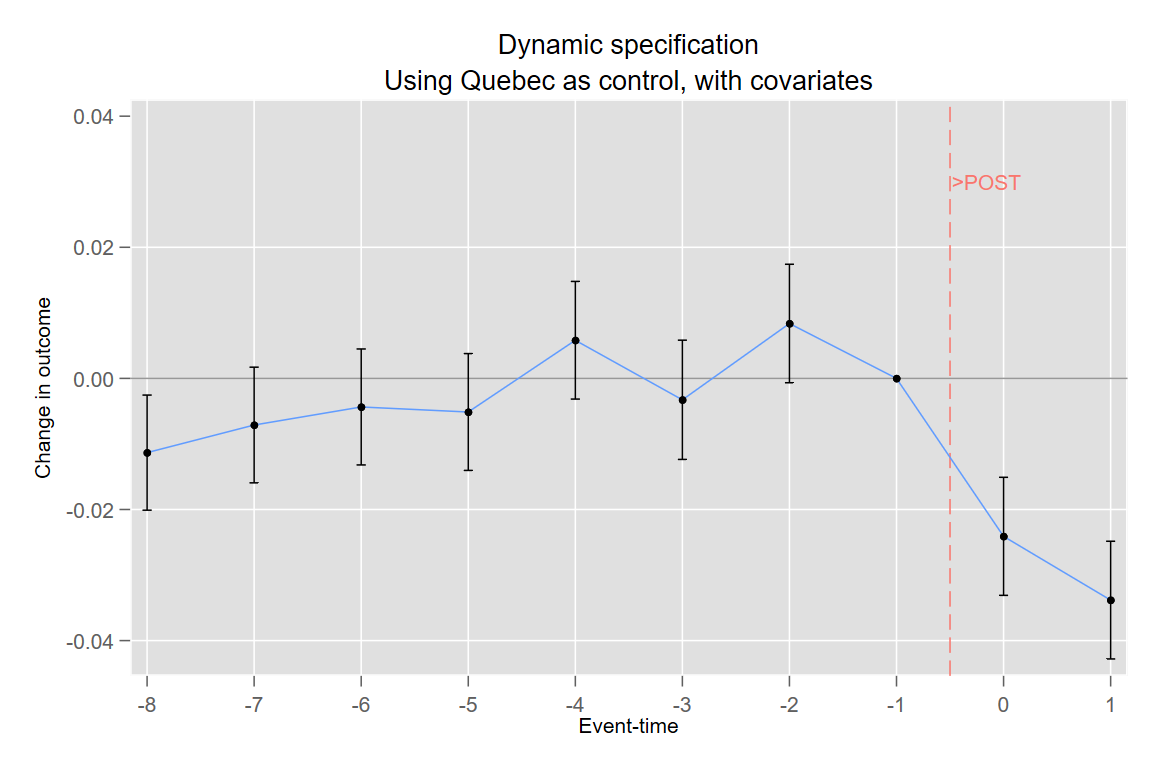
\includegraphics[keepaspectratio]{material/lecture-9/ontario5.png}}
\end{center}

\subsection{Alternate control group}\label{alternate-control-group}

Using Manitoba as a control, we see strong evidence of a violation of
parallel trends.

\begin{center}
\pandocbounded{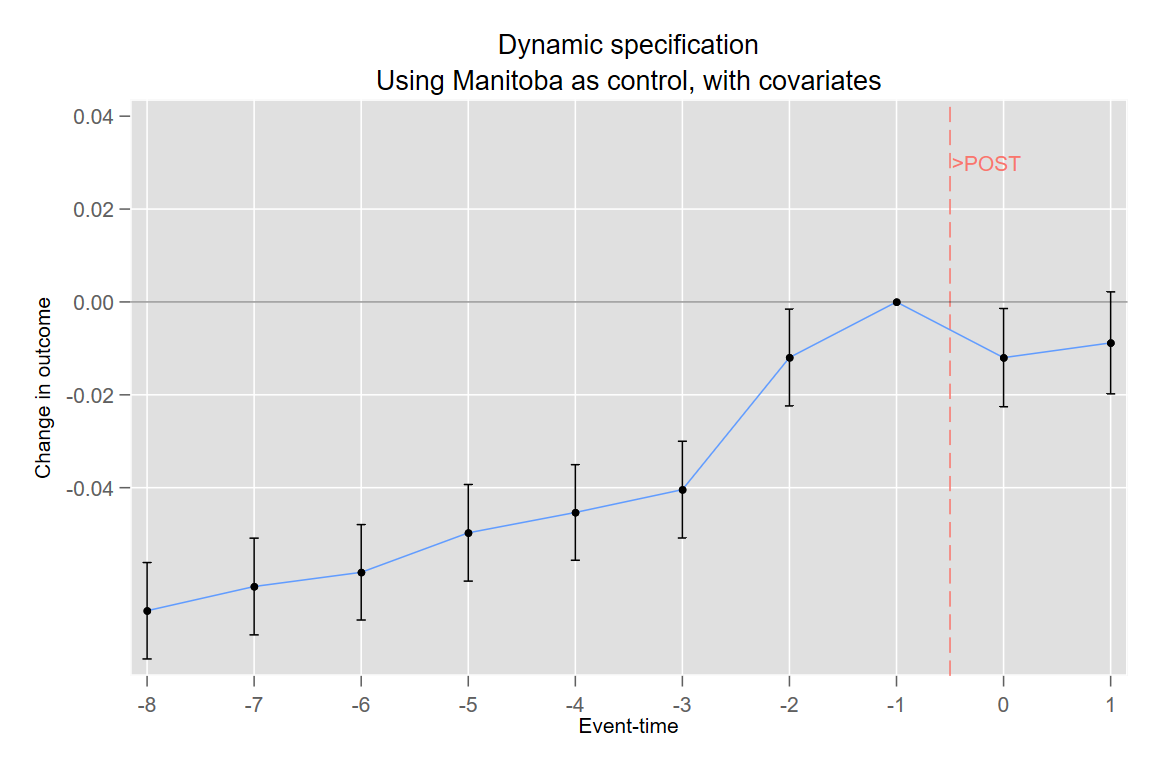
\includegraphics[keepaspectratio]{material/lecture-9/ontario6.png}}
\end{center}

\subsection{Placebo}\label{placebo}

We could examine whether there is an effect for older workers.

\begin{center}
\pandocbounded{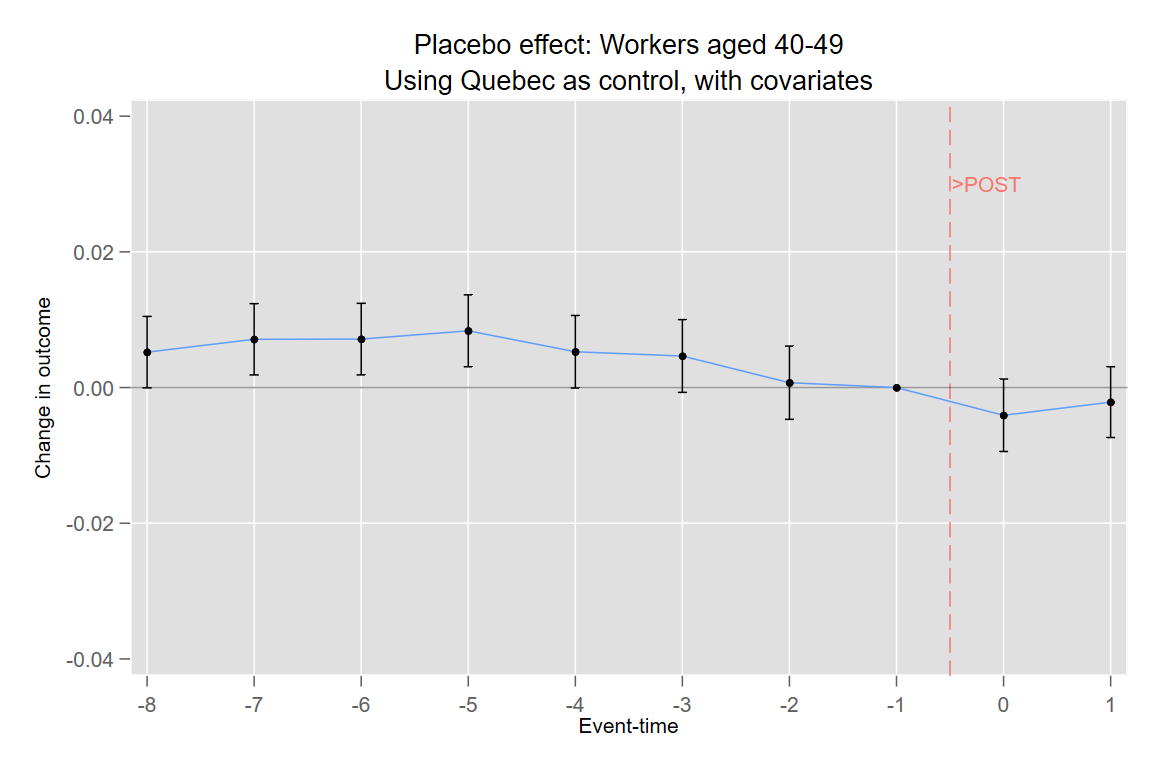
\includegraphics[keepaspectratio]{material/lecture-9/ontario7.png}}
\end{center}

\section{References}\label{references}

\subsection*{Bibliography}\label{bibliography}
\addcontentsline{toc}{subsection}{Bibliography}

\phantomsection\label{refs}
\begin{CSLReferences}{1}{0}
\bibitem[\citeproctext]{ref-card1994minimum}
Card, David, and Alan Krueger. 1994. {``Minimum Wages and Employment: A
Case Study of the New Jersey and Pennsylvania Fast Food Industries.''}
\emph{American Economic Review} 84 (4): 772--93.

\end{CSLReferences}




\end{document}
